\chapter{Accommodating QuDs: Qtrees}\label{chap:accommodating-quds}

This Chapter introduces a model of questions that is more sophisticated than standardly assumed (cf. Chapter \ref{chap:introduction}). Questions are defined as recursive partitions, or parse trees of the Context Set. This model is shown to capture fine-grained information about how questions relate to each other in terms of specificity, and what it means to answer a question. The Chapter then describes how such questions can be ``retro-engineered'' from assertions, in a compositional way. Lastly, we suggest how this model of questions can eventually make novel predictions in the domain of pragmatic oddness. 


\section{Making sense}

\subsection{Oddness despite relevance and informativeness}
In Chapter \ref{chap:introduction}, we have seen that assertive sentences should be informative, i.e. lead to an incremental shrinkage of the Context Set (\textbf{CS}) \citep{Stalnaker1978,Heim1982}. We have also seen that they should be relevant, i.e. shrink the CS in a way consistent with the Question under Discussion (\textbf{QuD}) \citep{Lewis1988,Roberts2012}. But sometimes, it is unclear what the QuD should be. For instance, the exchange in (\ref{ex:exchange-qud-settled}) already settles the overt QuD (\textit{Have you seen Jo today?}), and intersects the CS with the set of worlds in which Ed has not seen Jo on the day that \textit{today} refers to. But one could imagine many possible continuations to Ed's utterance. Any such continuation should be informative and relevant to \textit{some} QuD, but it is unclear how this QuD should be determined. In principle, it could be any non-vacuous partition of the newly updated CS. But there are many such partitions. How to know which one to pick?

\begin{exe}
	\ex {Al: Have you seen Jo today?\\
		Ed: No I haven't...}\label{ex:exchange-qud-settled}
\end{exe}

Let us consider the following felicitous follow-up to (\ref{ex:exchange-qud-settled}). This continuation is felicitous, so, should be both informative and relevant. To be relevant, the sentence has to relate to a QuD. But, as mentioned earlier, the overt QuD \textit{Have you seen Jo?} is at that point already settled. This suggests that, when no overt QuD is on the table, a ``reasonable'' QuD is chosen among all the possible non-vacuous partitions of the CS, and is such that the sentence under consideration properly answers it. This is motivated by the idea that sentences are never uttered in and of themselves; their purpose is to answer a question, overt or not, and to induce further questions \cite{Roberts1996}. A pragmatic model of assertion therefore needs to integrate what sentences mean, but also what kind of information structure they evoke. Assuming such a ``reasonable'' QuD is along the lines of \textit{Where is Jo?}, then, the continuation in (\ref{ex2:non-red-followup}) is predicted to be both informative (it says that Jo is sick or at a conference), and relevant.

\begin{exe}
	\ex {--Have you seen Jo today?\\
		--No I haven't... Either she is sick, or if she's not sick, she is at a conference.}\label{ex2:non-red-followup}
\end{exe}

But even if some implicit ``reasonable'' QuD can be inferred in the absence of an overt one, some cases of oddness remain mysterious. The follow-up sentence in (\ref{ex2:red-followup}) for instance, is equivalent to the one in (\ref{ex2:non-red-followup}) assuming implication is material, and so should in principle evoke the same QuD. (\ref{ex2:non-red-followup}) is thus predicted to be both informative and relevant, just like (\ref{ex2:non-red-followup}). Yet, this follow-up is sharply odd.

\begin{exe}
	\ex {--Have you seen Jo today?\\
		--No I haven't... \# Either she is sick, or if she's not at a conference, she is sick.}\label{ex2:red-followup}
\end{exe}

These two datapoints outline the following desideratum: if the contrast between (\ref{ex2:non-red-followup}) and (\ref{ex2:red-followup}) is due to the nature of the ``reasonable'' QuDs inferred from these sentences, then one must devise a way to systematically derive QuDs from out-of-the-blue assertions, in such a way that semantically similar, yet structurally distinct assertions, sometimes give rise to distinct QuDs.



This Chapter will address this desideratum and introduce a pragmatic model of these sentences in which (i) they package information differently in terms of their evoked QuDs, and (ii) unlike (\ref{ex2:red-followup}), (\ref{ex2:non-red-followup}), packages information in a way that is pragmatically optimal.

\subsection{Overview  and motivation of the Chapter}
The machinery we introduce in this Chapter aims to account for the above datapoints (among others), by relating their felicity or oddness to the QuD(s) inferred from them. The fundamental principle we want to operationalize is \textit{Question-Answer Congruence} (henceforth \textbf{QAC}), as formalized by \citet{Katzir2015},\footnote{This principle has been discussed in several forms for many years, within and outside the field of generative linguistics. See for instance \citet{Rooth1992} for a discussion on how focused assertions and questions can be systematically related in terms of their \textit{semantics}.} and given in (\ref{ex2:q-a-congruence}). 

\begin{exe}
	\ex {\textit{Question-Answer Congruence (\textbf{QAC}).} A felicitous assertion has to be a good answer to a good question.}\label{ex2:q-a-congruence}
\end{exe}

This take on QAC is interesting because it roots this principle in pragmatics, and is broad enough to encompass a variety of constraints that were previously not grouped under the same umbrella. Chapter \ref{chap:introduction} for instance, showed that \textsc{Relevance} could rule out a wide range of question-answer pairs, and as such could constitute a partial implementation of QAC. But QAC may in principle involve other constraints applying to question-answer pairs. This dissertation will show that, under a certain interpretation of ``good answer'' and ``good question'', many more cases of pragmatic oddness can be understood as an accross-the-board failure of QAC.

In this Chapter, we will lay out the groundwork for this more general pragmatic theory of question-answer well-formedness. We begin by introducing a more new model of questions, based on nested partitions, instead of mere partitions of the CS (as discussed in Chapter \ref{chap:introduction}). This model is building on \citet{Buring2003,Ippolito2019,Zhang2022}, among many others. Next, equipped with this model of questions, we will show that questions can be evoked by assertions in a compositional way. As a result, sentences involving different operators (specifically, disjunctions and conditionals), give rise to different kinds of questions. Crucially in this model, each sentence may be associated with multiple potential questions. Finally, we will sketch what a pragmatics for question-answer pairs should look like in that framework. In line with QAC, a sentence which cannot be felicitously paired with \textit{any} question will be deemed odd. This can happen if \textit{all} the pairs formed by a sentence and a question it evokes, are themselves ill-formed. 

We now proceed to define questions, not just as partition, but rather, as parse trees of the Context Set, that we will call Qtrees.

\section{Structure of Question Trees}

\subsection{From partitions to recursive partitions, to parse trees}\label{sec:nested-partition}
Building on the standard model presented in Chapter \ref{chap:introduction}, we introduce a more elaborate view of the pragmatics of questions. This model will incorporate the idea that questions have internal structure, and specifically, are hierarchically organized. This hierarchical organization is meant to capture the intuition that a question such as (\ref{ex2:city-question}) for instance, appears more \textit{fine-grained}, than a question like (\ref{ex2:country-question}). Alternatively, whatever proposition identifies a cell in (\ref{ex2:city-question}), also identifies a cell in (\ref{ex2:country-question}). Crucially, this intuition will be incorporated in the pragmatics of questions, and so will be made directly accessible to the grammar.

\begin{exe}
	\ex 
	\begin{xlist}
		\ex {In which city did Jo grow up?}\label{ex2:city-question}
		\ex {In which country did Jo grow up?}\label{ex2:country-question}
	\end{xlist}
\end{exe}

First, let us observe that these intuitions about question-specificity are \textit{not} readily cashed out by standard partitions or alternative sets associated with questions. (\ref{ex2:city-question})'s and (\ref{ex2:country-question})'s sets of alternatives, given in (\ref{ex2:city-partition}) and (\ref{ex2:country-partition}) respectively, are made of disjoint, non empty propositions which, at a certain level of approximation, cover the space of all possibilities.\footnote{We will assume here, that any point on Earth is associated with one single country, and one single city, in a Voronoi fashion. At this level of approximation, there is no countryless or cityless area. Alternatively, one could assume that there are cityless areas, but that the possibility of Jo growing up in such areas is ruled-out by the presupposition carried by \textit{which}-questions like (\ref{ex2:city-question}). Under this assumption, \textit{where}-questions may require more work.} In other words, these alternatives already partition the set of \textit{all} worlds. The partition that (\ref{ex2:city-partition}) (resp. (\ref{ex2:country-partition})) induces on the CS is therefore obtained from (\ref{ex2:city-partition}) (resp. (\ref{ex2:country-partition})) by simply intersecting each of its elements (a proposition/cell) with the CS--discarding empty sets.

\begin{exe}
	\ex 
	\begin{xlist}
		\ex {$\llbracket$ In which city did Jo grow up?$\rrbracket^w$ =\\$\lbrace p \ | \ \exists l. \ \text{$l$ is a city} \wedge p = \lambda w'. \ \text{Jo grew up in $l$ in $w'$}\rbrace$}\label{ex2:city-partition}
		\ex {$\llbracket$ In which country did Jo grow up?$\rrbracket^w$ =\\$\lbrace p \ | \ \exists l. \ \text{$l$ is a country} \wedge p = \lambda w'. \ \text{Jo grew up in $l$ in $w'$}\rbrace$}\label{ex2:country-partition}
	\end{xlist}
\end{exe}

(\ref{ex2:city-question}) therefore induces a by-city partition of the CS (see Figure \ref{fig2:city-partition}), while (\ref{ex2:country-question}) induces a by-country partition (see Figure \ref{fig2:country-partition}). But nothing in (\ref{ex2:city-question})'s partition signals that each of its cells is properly contained in a cell of (\ref{ex2:country-question})'s partition. This property can de derived from the two structures, but is not readily \textit{encoded} by them.



\begin{figure}[H]
	\centering
	\begin{subfigure}[t]{.48\linewidth}
		\centering
		\scalebox{1.25}{
		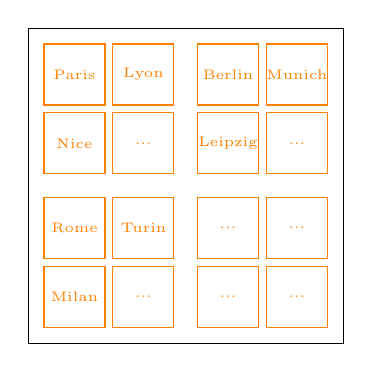
\begin{tikzpicture}	
			\draw [draw=black] (0, 0) rectangle (4,4) ;
			\draw [draw=orange] (0.2, 2.15) rectangle (0.975, 2.925) node[pos=.5] {\tiny \textcolor{orange}{Nice}};
			\draw [draw=orange] (1.075, 2.15) rectangle (1.85, 2.925) node[pos=.5] {\tiny \textcolor{orange}{...}};
			\draw [draw=orange] (0.2, 3.025) rectangle (0.975, 3.8) node[pos=.5] {\tiny \textcolor{orange}{Paris}};
			\draw [draw=orange] (1.075, 3.025) rectangle (1.85, 3.8) node[pos=.5] {\tiny \textcolor{orange}{Lyon}};
			\draw [draw=orange] (0.2, 0.2) rectangle (0.975, 0.975) node[pos=.5] {\tiny \textcolor{orange}{Milan}};
			\draw [draw=orange] (1.075, 0.2) rectangle (1.85, 0.975) node[pos=.5] {\tiny \textcolor{orange}{...}};
			\draw [draw=orange] (0.2, 1.075) rectangle (0.975, 1.85) node[pos=.5] {\tiny \textcolor{orange}{Rome}};
			\draw [draw=orange] (1.075, 1.075) rectangle (1.85, 1.85) node[pos=.5] {\tiny \textcolor{orange}{Turin}};
			
			\draw [draw=orange] (2.15, 0.2) rectangle (2.925, 0.975) node[pos=.5] {\tiny \textcolor{orange}{...}};
			\draw [draw=orange] (3.025, 0.2) rectangle (3.8, 0.975) node[pos=.5] {\tiny \textcolor{orange}{...}};
			\draw [draw=orange] (2.15, 1.075) rectangle (2.925, 1.85) node[pos=.5] {\tiny \textcolor{orange}{...}};
			\draw [draw=orange] (3.025, 1.075) rectangle (3.8, 1.85) node[pos=.5] {\tiny \textcolor{orange}{...}};
			
			\draw [draw=orange] (2.15, 2.15) rectangle (2.925, 2.925) node[pos=.5] {\tiny \textcolor{orange}{Leipzig}};
			\draw [draw=orange] (3.025, 2.15) rectangle (3.8, 2.925) node[pos=.5] {\tiny \textcolor{orange}{...}};
			\draw [draw=orange] (2.15, 3.025) rectangle (2.925, 3.8) node[pos=.5] {\tiny \textcolor{orange}{Berlin}};
			\draw [draw=orange] (3.025, 3.025) rectangle (3.8, 3.8) node[pos=.5] {\tiny \textcolor{orange}{Munich}};
		\end{tikzpicture}}
		\caption{By-city partition associated with (\ref{ex2:city-partition}). Cells are ordered on a grid for clarity only.}\label{fig2:city-partition}
	\end{subfigure}\hfill
	\begin{subfigure}[t]{.48\linewidth}
		\centering
		\scalebox{1.25}{
		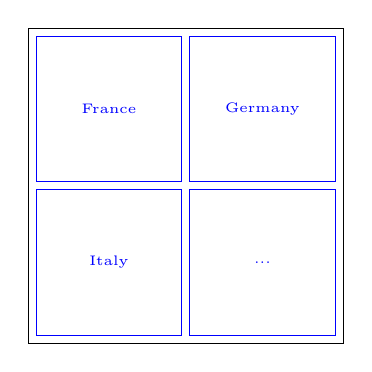
\begin{tikzpicture}	
			\draw [draw=black] (0, 0) rectangle (4,4);
			\draw [draw=blue] (0.1, 2.05) rectangle (1.95, 3.9) node[pos=.5] {\tiny \textcolor{blue}{France}};
			\draw [draw=blue] (2.05, 0.1) rectangle (3.9, 1.95) node[pos=.5] {\tiny \textcolor{blue}{...}};
			\draw [draw=blue] (0.1, 0.1) rectangle (1.95, 1.95) node[pos=.5] {\tiny \textcolor{blue}{Italy}};
			\draw [draw=blue] (2.05, 2.05) rectangle (3.9, 3.9) node[pos=.5] {\tiny \textcolor{blue}{Germany}};
		\end{tikzpicture}}
		\caption{By-country partition associated with (\ref{ex2:country-partition}). Cells are ordered on a grid for clarity only.}\label{fig2:country-partition}
	\end{subfigure}
	\caption{Standard partitions induced by a fine-grained (\ref{ex2:city-partition}) and a coarser-grained question (\ref{ex2:country-partition}).}
\end{figure}

Intuitively, grouping together the propositions listed in (\ref{ex2:city-partition}) talking about cities belonging to the same country, would help capture the desired property. This is done in (\ref{ex2:city-parse}). (\ref{ex2:city-parse}) then defines a set of sets of propositions. 
\begin{exe}
	\ex {$\llbracket$ In which city did Jo grow up?$\rrbracket^w$ =\\$\lbrace\lbrace p \ | \ \exists l. \ \text{$l$ is a city in $l'$} \wedge \ p = \lambda w'. \ \text{Jo grew up in $l$ in $w'$}\rbrace \ | \ l' \text{ is a country} \rbrace$}\label{ex2:city-parse}
\end{exe}

Grouping together cells within bigger sets (which are cells themselves), amounts to building a \textit{nested} partition of the CS. In our example, the ``outer'' partition is by-country, and the ``inner'' partition, is by-city. Graphically, this is equivalent to adding the ``blue rectangles'' from Figure \ref{fig2:country-partition}, to Figure \ref{fig2:city-partition}. This operation is performed in Figure \ref{fig2:city-recursive-partition}. The tree in Figure \ref{fig2:city-tree} is yet another, more readable way to represent the same thing. In this tree, each node refers to a proposition of the form \textit{Jo grew up in l}, $l$ denoting a city or a country. Each node is understood as intersected with the CS, which corresponds to the root of the tree. Therefore, each node forms a proper subset of the CS. Nodes appearing at the same level (forming a ``layer''), partition the CS. Deeper layers, correspond to finer-grained partitions. Tree like Figure \ref{fig2:city-tree} will be used throughout the dissertation to represent nested partitions like Figure \ref{fig2:city-recursive-partition}. One must always keep in mind that the two representations are equivalent. (\ref{ex2:set-tree-bijection}) formally defines the bijective mapping between nested sets of propositions (dubbed \textit{inductive propositions}) like (\ref{ex2:city-parse}), and tree structures like Figure \ref{fig2:city-tree}.

\begin{figure}[H]
	\centering
	\begin{subfigure}[t]{.45\linewidth}
		\centering
		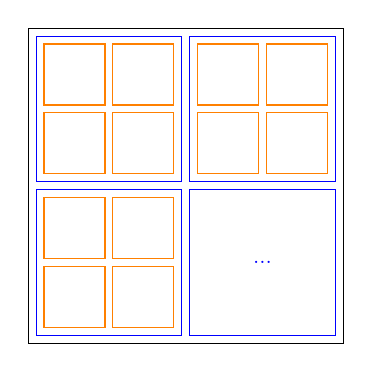
\begin{tikzpicture}	
			\draw [draw=black] (0, 0) rectangle (4,4) ;
			\draw [draw=blue] (0.1, 2.05) rectangle (1.95, 3.9);
				\draw [draw=orange] (0.2, 2.15) rectangle (0.975, 2.925);
				\draw [draw=orange] (1.075, 2.15) rectangle (1.85, 2.925);
				\draw [draw=orange] (0.2, 3.025) rectangle (0.975, 3.8);
				\draw [draw=orange] (1.075, 3.025) rectangle (1.85, 3.8);
			\draw [draw=blue] (2.05, 0.1) rectangle (3.9, 1.95) node[pos=.5] {\scriptsize \textcolor{blue}{...}};
			\draw [draw=blue] (0.1, 0.1) rectangle (1.95, 1.95);
				\draw [draw=orange] (0.2, 0.2) rectangle (0.975, 0.975);
				\draw [draw=orange] (1.075, 0.2) rectangle (1.85, 0.975);
				\draw [draw=orange] (0.2, 1.075) rectangle (0.975, 1.85);
				\draw [draw=orange] (1.075, 1.075) rectangle (1.85, 1.85);
			\draw [draw=blue] (2.05, 2.05) rectangle (3.9, 3.9);
				\draw [draw=orange] (2.15, 2.15) rectangle (2.925, 2.925);
				\draw [draw=orange] (3.025, 2.15) rectangle (3.8, 2.925);
				\draw [draw=orange] (2.15, 3.025) rectangle (2.925, 3.8);
				\draw [draw=orange] (3.025, 3.025) rectangle (3.8, 3.8);
		\end{tikzpicture}
		\caption{Recursive partition view}\label{fig2:city-recursive-partition}
	\end{subfigure}
	\hfill
	\begin{subfigure}[t]{.5\linewidth}
		\centering
		\vspace{-4.4cm}
		\begin{forest}
			[{CS\\
				Jo grew up in...}[\textcolor{blue}{France}[\textcolor{orange}{{Paris}}][\textcolor{orange}{Lyon}][\textcolor{orange}{...}]][\textcolor{blue}{Germany}[\textcolor{orange}{Berlin}][\textcolor{orange}{...}]][\textcolor{blue}{Italy}[\textcolor{orange}{...}]][\textcolor{blue}{...}]]
		\end{forest}
		\caption{Tree view}\label{fig2:city-tree}
	\end{subfigure}
	\caption{Alternative representations of the CS corresponding to the nested sets of (\ref{ex2:city-parse}).}\label{tree:country-city-parse}
\end{figure}


\begin{exe}
	\ex {\textit{Set-to-tree bijection. } To define this bijection, we first define inductive propositions, and their propositional content. $S$ is an inductive proposition if either:
		\begin{itemize}
			\item $S$ is a set of worlds (i.e. a proposition);
			\item $S$ is a set of inductive propositions.
		\end{itemize}
		The propositional content of an inductive proposition is then defined as:
		\begin{itemize}
			\item If $S$ is a proposition: $S$;
			\item If $S$ is a set of inductive propositions: the grand union of the propositional contents of $S$'s elements.
		\end{itemize}
		Any inductive proposition $S$ is in a bijection with a tree structure whose nodes are propositions, and defined as:
		\begin{itemize}
			\item If $S$ is a proposition: the tree node denoting $S$;
			\item If $S$ is a set of inductive propositions: the tree whose root denotes $S$'s propositional content, and whose children are the tree structures induced by each of $S$'s elements. 
	\end{itemize}}\label{ex2:set-tree-bijection}
\end{exe}

So far, we have shown that the standard view linking questions to partitions, fails to account for the intuition that questions differing in terms of specificity, stand in some kind of inclusion relation encoded in their structure. We proposed a way to cash out this intuition, by appealing to recursive partitions, that we represent as trees for clarity.


We now proceed to generalize these observations about the structure of questions. Building on \citet{Buring2003,Riester2019,Onea2016,Ippolito2019,Zhang2022} (among others), we take questions to denote \textit{parse trees} of the CS, i.e. structures that hierarchically organize the worlds of the CS. Such trees (abbreviated \textbf{Qtrees}) are defined in (\ref{ex2:qtree-def}). 
%(\ref{ex2:parse-def}) provide a more general definition of a parse.\footnote{This slightly differs from the notion of parse defined for sentences for instance, in which linear precedence must be preserved.} 
\begin{exe}
	\ex {\textit{Structure of Question-trees (\textbf{Qtrees}).} Qtrees are rooted trees whose nodes are all subsets of the CS and s.t.:
		\begin{itemize}
			\item Their root generally\footnote{In the case of sentences carrying presuppositions, the root will be assumed to correspond to the intersection between the CS and the sentence's presupposition. In fact, the whole Qtree will be nodewise intersected with the presupposition. This will be put to use in Chapters \ref{chap:scalarity} and \ref{chap:exh-incr}. But the examples we will see before this, will all involve Qtree rooted in the CS.} refers to the CS;
			\item Any intermediate node is a proposition, which is partitioned by the set of its children.
		\end{itemize}
	}\label{ex2:qtree-def}
\end{exe}
%	\ex {\textit{Parse.} Let $S$ be a set. A parse of $S$ is a rooted tree whose nodes are subsets of $S$ and s.t.:
%		\begin{itemize}
%			\item The root is $S$;
%			\item Any intermediate node is partitioned by the set of its children.
%		\end{itemize}
%	}\label{ex2:parse-def}

A Qtree can be bijectively mapped to a nested partition of the CS as defined in (\ref{ex:nested-partition}). Due to this equivalence, we will mostly use Qtrees in the rest of this dissertation.

\begin{exe}
	\ex {\textit{Nested partition.} A nested partition $P$ of a set $S$ is a kind of inductive proposition, s.t.:
		\begin{itemize}
			\item If $P$ is a set of inductive propositions, then the propositional contents of $P$'s elements partition $P$'s propositional content. Additionally, $P$'s elements are nested partitions of their own propositional content. 
		\end{itemize}	
	}\label{ex:nested-partition}
\end{exe}


Before investigating the interpretation and the structural properties of model of questions, the next Section covers a few core concepts from graph theory that will be useful in the rest of the Chapter and beyond.


\subsection{A brief refresher on graph theory (and a few useful concepts for Qtrees)}

(\ref{ex2:qtree-def}) defines Qtres as rooted trees. Linguists typically understand trees as relations between parent nodes and their children, along the lines of (\ref{ex2:recursive-interpretation}).

\begin{exe}
	\ex {\textit{Rooted tree (inductive version).} A tree rooted in $N$ is either:
		\begin{itemize}
			\item $N$ (single, childless node);
			\item $N$, along with $N$'s children, which are all rooted trees.
	\end{itemize}}\label{ex:tree-inductive}
\end{exe}

But we will see throughout this dissertation that it is also useful to see a tree as a specific kind of graph. We will first define graphs, then define trees as a subkind of graph, and lastly, show the importance of defining a root in such trees. The definition of a graph is given in (\ref{ex:graph}). A graph is a way to represent a binary relation, which by default will be symmetric\footnote{\textit{Undirected} graphs, that we will simply call graphs, implement symmetric relations, while \textit{directed} graphs implement asymmetric relations.}. Elements in the domain of the relation are modeled as nodes, and unordered pairs of nodes are connected with an edge, iff they verify the relation. A graph therefore amounts to a set of nodes, and a set of edges between these nodes. This is illustrated in Figure \ref{fig:basic-graph}.

\begin{exe}	
	\ex {\textit{Graph.} A graph is defined by a set of nodes $\mathcal{N}$ and by a set of edges $\mathcal{E}$ between elements of $\mathcal{N}$. Edges are defined as unordered pairs of nodes: $\mathcal{E} \subseteq \lbrace \lbrace N_1, N_2\rbrace \ | \ (N_1, N_2) \in \mathcal{N}^2\rbrace$}\label{ex:graph}
\end{exe}

\begin{figure}[H]
	\centering
	\begin{tikzpicture}
		\node[shape=circle,draw=black] (A) at (0,0) {A};
		\node[shape=circle,draw=black] (B) at (0,3) {B};
		\node[shape=circle,draw=black] (C) at (2.5,4) {C};
		\node[shape=circle,draw=black] (D) at (2.5,1) {D};
		\node[shape=circle,draw=black] (F) at (5,3) {F} ;
		\node[shape=circle,draw=black] (E) at (-2,2) {E} ;
		
		\path [-,color=orange] (A) edge node[left] {} (B);
		\path [-](B) edge node[left] {} (C);
		\path [-,color=orange](A) edge node[left] {} (D);
		\path [-](D) edge node[left] {} (C);
		\path [-,color=orange](D) edge node[right] {} (F);   
	\end{tikzpicture}
	\caption{A graph $G=(\mathcal{N}, \mathcal{E})$, with $\mathcal{N}=\lbrace A, B, C, D, E, F\rbrace$ and $\mathcal{E}=\lbrace \lbrace A, B\rbrace, \lbrace A, D\rbrace, \lbrace B, C\rbrace, \lbrace C, D\rbrace, \lbrace D, F\rbrace\rbrace$.}\label{fig:basic-graph}
\end{figure}

This definition allows to define rooted trees as a kind of graph with a few extra properties: connectivity, acyclicity, and rootedness; see (\ref{ex:rooted-tree}). We now unpack what these three extra properties mean for graphs. This will lead us to define a few useful concepts applying to trees, namely paths, ancestry, and depth.

\begin{exe}
	\ex {\textit{Rooted tree (graph version).} A rooted tree is a graph that is connected and acyclic, and features a distinguished node called root.}\label{ex:rooted-tree}
\end{exe}

In graphs, sequences of adjacent edges form paths. For instance, in Figure \ref{fig:basic-graph}, the ordered sequence $[$\textcolor{orange}{$\lbrace A, B\rbrace$}, \textcolor{orange}{$\lbrace A, D\rbrace$}, \textcolor{orange}{$\lbrace D, F\rbrace$}$]$ forms a path, between node $A$ and node $F$. This is generalized in (\ref{ex:graph-path}).

\begin{exe}
	\ex {\textit{Path.} Let $G = (\mathcal{N}, \mathcal{E})$ be a graph. Let $(N_1, N_2) \in \mathcal{N}^2$ be two nodes of $G$. There is a path in $G$ between $N_1$ and $N_2$ (abbreviated $N_1 \stackrel{G}{\leadsto}  N_2$) iff $N_1$ and $N_2$ can be connected by a series of edges in $G$, i.e. $\exists (e_1, ... e_k) \in \mathcal{E}^k. \ N_1 \in e_1 \wedge N_2 \in e_k \wedge \forall i \in [1; k-1]. \  |e_i \cap e_{i+1}|  = 1$, where $|.|$ is the cardinality operator.}\label{ex:graph-path}
\end{exe}

In Figure \ref{fig:basic-graph}, it is easy to see that nodes $A$, $B$, $C$, $D$ and $F$ are all connected to each other by at least one path (in fact, infinitely many of them that cycle through these nodes). Node $E$ on the other hand, is isolated. So, Figure \ref{fig:basic-graph} represents a graph that is \textit{not} connected. If $E$ were removed from the set of nodes, and the edges remained the same, the resulting graph would be connected. This concept of connectivity is generalized in (\ref{ex:graph-connectivity}). If a graph is a tree, then, it is connected.
\begin{exe}
	\ex {\textit{Connectivity.} Let $G = (\mathcal{N}, \mathcal{E})$ be a graph. $G$ is connected, iff there is a path in $G$ between any pair of nodes in $\mathcal{N}$, i.e. $\forall (N_1, N_2) \in \mathcal{N}^2. \ N_1 \stackrel{G}{\leadsto} N_2$.}\label{ex:graph-connectivity}
\end{exe}

Another thing to note about Figure \ref{fig:basic-graph}, is that nodes $A$, $B$, $C$, and $D$ form a ``cycle'', there is a path that starts at one of these nodes (e.g., $C$), and ends at this very same node, \textit{via} $B$, $A$, and $D$. Because of this cycle, there are infinitely many paths between $A$, $B$, $C$, and $D$, and also between each of these nodes, and $F$. Removing the edge between, say, $A$ and $B$, would break the cycle (yet, interestingly, maintain connectivity between $A$, $B$, $C$, and $D$). The resulting graph would be acyclic. The general definition of an acyclic graph, is given in (\ref{ex:graph-acyclic}). If a graph is a tree, then, it is acyclic. Moreover, connectivity and acyclicity, are necessary and sufficient for a graph to be a tree.

\begin{exe}
	\ex {\textit{Acyclicity.} Let $G = (\mathcal{N}, \mathcal{E})$ be a graph. $G$ is acyclic, iff no node $N$ of $\mathcal{N}$ is s.t. there is a path starting and ending at $N$ in $G$, i.e. $\neg\exists N \in \mathcal{N}. \ N \stackrel{G}{\leadsto} N$.}\label{ex:graph-acyclic}
\end{exe}

We now have a definition of what kind of data structure a tree is. But why do we need  Qtrees to be ``rooted''? To understand why, let us go back to the tree in Figure \ref{fig2:city-tree}, repeated in Figure \ref{fig2:city-tree-repeated} below. The way this tree is represented on paper, is somehow misleading. Recall that, from the point of view of graph theory, a tree is just an undirected graph, with a few extra properties constraining its edges. If the tree represented in Figure \ref{fig2:city-tree-repeated} were not ``rooted'', nothing would prevent us from representing it in the form of Figure \ref{fig2:city-tree-france-root}: the nodes and edges are strictly the same, but in Figure \ref{fig2:city-tree-france-root}, \textit{France} ``appears'' to be the root of the tree, because visually, it is represented at the top. To avoid this confusion, the fact that the CS node should be ``at the top'' is made part of the representation of the tree--which then becomes a \textit{rooted} tree. So, a rooted tree is just a tree, plus one distinguished node that serves as root.

\begin{figure}[H]
	\centering
	\begin{subfigure}[t]{.45\linewidth}
		\centering
		\begin{forest}
			[{CS\\
				Jo grew up in...}[\textcolor{blue}{France}[\textcolor{orange}{{Paris}}][\textcolor{orange}{Lyon}][\textcolor{orange}{...}]][\textcolor{blue}{Germany}[\textcolor{orange}{Berlin}][\textcolor{orange}{...}]][\textcolor{blue}{Italy}[\textcolor{orange}{...}]][\textcolor{blue}{...}]]
		\end{forest}
		\caption{The ``intuitive'' view, in which the CS appears at the top.}\label{fig2:city-tree-repeated}
	\end{subfigure}
	\hfill
	\begin{subfigure}[t]{.45\linewidth}
		\centering
		\begin{forest}
			[\textcolor{blue}{France}[\textcolor{orange}{Paris}][\textcolor{orange}{Lyon}][\textcolor{orange}{...}][CS[\textcolor{blue}{Germany}[\textcolor{orange}{Berlin}][\textcolor{orange}{...}]][\textcolor{blue}{Italy}[\textcolor{orange}{...}]][\textcolor{blue}{...}]]]
		\end{forest}
		\caption{An alternative ``counter-intuitive'' view, in which the CS is \textit{not} at the top, yet all edges and nodes are the same.}\label{fig2:city-tree-france-root}
	\end{subfigure}
	\caption{Two equivalent ways to represent the tree corresponding to the question in (\ref{ex2:city-question}); assuming trees were connected, acyclic graphs, but not rooted.}
\end{figure}


The notion of a distinguished root in fact allows to define a few interesting properties on trees that linguist may be more familiar with, and that will be used throughout this dissertation. First, once a tree is rooted, it is possible to define a measure of distance between each node of the tree, and the root. This corresponds to the concept of depth, defined in (\ref{ex:tree-node-depth}). In Figure \ref{fig2:city-tree-repeated} for instance, the CS has depth $0$, \textit{Germany} depth $1$, and \textit{Lyon} depth $2$. This also allows to define the global ``size'' of the tree, in the form of its maximal depth; see (\ref{ex:tree-depth}). Figure \ref{fig2:city-tree-repeated} for instance, is a tree of depth $2$.

\begin{exe}
	\ex
	\begin{xlist}	
		\ex {\textit{Depth of a node in a rooted tree.} Let $T = (\mathcal{N}, \mathcal{E}, R)$ be a rooted tree, with root $R$. Let $N \in \mathcal{N}$. The depth of $N$ in $T$ ($d(N, T)$) corresponds to the length of the minimal path between $R$ and $N$ if $N \neq R$,\footnote{This path can be determined using a simple Depth-First Search algorithm starting from the root.} and is set to $0$ if $N = R$.}\label{ex:tree-node-depth}
		\ex {\textit{Depth of a rooted tree.} Let $T = (\mathcal{N}, \mathcal{E}, R)$ be a rooted tree, with root $R$. The depth of $T$ ($d(T)$) is the maximal depth of a node in $T$: $d(T) = max_{N \in \mathcal{N}}(d(N, T))$.}\label{ex:tree-depth}
	\end{xlist}
\end{exe}

Having a distinguished root, and the derived concepts of depth, gives us the parent-child relation between nodes for free.\footnote{in the next Section, we will introduce another definition of tree, that takes this relation as a primitive} This relation is defined based on depth and edges in (\ref{ex:parent-child}), and its transitive closure (the ancestor relation) is defined in (\ref{ex:ancestor}), in two possible ways. 

\begin{exe}
	\ex {\textit{Parent-child relation in a rooted tree.} Let $T = (\mathcal{N}, \mathcal{E}, R)$ be a rooted tree. Let $(N_1, N_2) \in \mathcal{N}^2$. $N_1$ is the parent of $N_2$  (and $N_2$ is the child of $N_1$), iff $\lbrace N_1, N_2\rbrace \in \mathcal{E}$ and $d(N_1, T) < d(N_2, T)$.}\label{ex:parent-child}
	\ex\label{ex:ancestor}
	\begin{xlist}
		\ex {\textit{Ancestor relation (recursive version).} Let $T = (\mathcal{N}, \mathcal{E}, R)$ be a rooted tree. Let $(N_1, N_2) \in \mathcal{N}^2$. $N_1$ is an ancestor of $N_2$ iff either:
			\begin{itemize}
				\item $N_1$ is the parent of $N_2$;
				\item or $N_1$ is the parent of an ancestor of $N_2$.
		\end{itemize}}
	\ex {\textit{Ancestor relation (path version).} Let $T = (\mathcal{N}, \mathcal{E}, R)$ be a rooted tree. Let $(N_1, N_2) \in \mathcal{N}^2$. $N_1$ is an ancestor of $N_2$ iff $N_1 \stackrel{T}{\leadsto} N_2$ and $d(N_1, T) < d(N_2, T)$.}
	\end{xlist}
\end{exe}

Lastly, in the rest of this dissertation, we will extensively use the concept of \textit{layer}, that we define as a the maximal set of same-depth nodes in a rooted tree; see (\ref{ex:tree-layer}). Figure \ref{fig2:city-tree-repeated} features a country-layer at depth $1$, and a city-layer at depth $2$. Layers therefore reflect an intuitive notion of granularity.

\begin{exe}
	\ex {\textit{Depth-$k$ layer of a rooted tree.} Let $T = (\mathcal{N}, \mathcal{E}, R)$ be a rooted tree, with root $R$. Let $k$ be an integer s.t. $0\geq k<d(T)$. The depth-$k$ layer of $T$ is the set of nodes in $\mathcal{N}$ whose depth is $k$, i.e. $\lbrace N \in \mathcal{N} \ | \ d(N, T)=k\rbrace$.}\label{ex:tree-layer}
\end{exe}


Now that we have defined the core structure of Qtrees along with a few related properties and metrics, we proceed to assign an interpretation to this kind of structure.

\subsection{Interpreting Qtrees}\label{sec:interpreting-qtrees}
At the end of Section \ref{sec:nested-partition}, we showed that question should better be represented as nested partition, in order to encode their degree of specificity, and the grammar sensitive to how more or less fine-grained questions relate to each other. We also discussed how nested partitions could be unequivocally represented as Qtrees. It is easy to see that the tree in Figure \ref{fig2:city-tree}/\ref{fig2:city-tree-repeated}, repeated again in Figure \ref{fig2:city-qtree}, is a Qtree according to (\ref{ex2:qtree-def}). We saw that this Qtree intuitively capture the idea that a \textit{Which country?} kind of question, is contained in a \textit{Which city?} kind of question. We now investigate how to exploit this hierarchy in a meaningful way. We will use Figure \ref{fig2:city-qtree} as an example, and now assign an interpretation to nodes and paths in such structures. We will focus on three meaningful aspects of Qtrees: answer-granularity (understood as node depth), strategies of inquiry (understood as paths), and question refinement (understood as tree inclusion)

\begin{figure}[H]
	\centering
	\begin{forest}
		[{CS\\
			Jo grew up in...}[\textcolor{blue}{France}[\textcolor{orange}{{Paris}}][\textcolor{orange}{Lyon}][\textcolor{orange}{...}]][\textcolor{blue}{Germany}[\textcolor{orange}{Berlin}][\textcolor{orange}{...}]][\textcolor{blue}{Italy}[\textcolor{orange}{...}]][\textcolor{blue}{...}]]
	\end{forest}
	\caption{``Intuitive'' Qtree for \textit{Which city did Jo grow up in?}}\label{fig2:city-qtree}
\end{figure}

We start with the interpretation of nodes as possible answers, with different granularities. The root of Figure \ref{fig2:city-qtree} for instance, which corresponds to the entire CS, defines a tautology: it is a proposition which is true of all worlds of the CS, because it simply coincides with it.\footnote{Chapter \ref{chap:introduction} moreover identifies it as an uninformative proposition that is Lewis-relevant but not Roberts-relevant.} It can be understood as identifying the unique cell of coarsest-grained partition of the CS, that is, the CS itself. By contrast, leaves like \textit{Paris}, \textit{Lyon}, \textit{Berlin} in Figure \ref{fig2:city-qtree}, correspond to the ``smallest'' cells of the recursive partition that the Qtree defines. They can be seen as maximal answer to the underlying question, e.g., \textit{In which city did Jo grow up?}. Intermediate nodes like \textit{France} or \textit{Germany} in Figure \ref{fig2:city-qtree}, form cells of ``intermediate'' size, and can always be seen as unions of leaves. They appear to correspond to non-maximal answers. Because Qtrees can be made of many layers, they induce a hierarchy between non-maximal answers: an non-maximal answer $p$ is ``more maximal'' than another non-maximal answer $q$, iff the node corresponding to $p$ is located deeper in the Qtree than the node corresponding to $q$. This is formalized in (\ref{ex2:answer-gran}).

\begin{exe}
	\ex {\textit{Answer granularity.} Let $T$ be a Qtree and $(N_1, N_2)$ be two nodes in $T$. $N_1$ constitutes a finer-grained answer than $N_2$ iff $d(N_1, T) > d(N_2, T)$. This implies that leaves of $T$ correspond to the finest-grained answers (maximal answers) to the question $T$ represents.}\label{ex2:answer-gran}
\end{exe}


Next, we discuss how Qtree encapsulate \citeauthor{Roberts1996}'s notion of \textit{Strategy of Inquiry}. To this end, we observe that nodes in a tree can receive a ``recursive'' interpretation, that incorporates everything the node dominates. Under this interpretation, a node $N$ in a Qtree is not only what $N$ denotes; it is the whole subtree ($\sim$subquestion) rooted in $N$, as defined in (\ref{ex2:recursive-interpretation})


\begin{exe}
	\ex\label{ex2:recursive-interpretation} {\textit{Recursive interpretation of tree nodes}. Let $T = (\mathcal{N}, \mathcal{E}, R)$ be a rooted tree. Let $N \in \mathcal{N}$ be a node of $T$. $N$'s recursive interpretation corresponds to:
		\begin{itemize}
			\item $N$, if $N$ is a leaf;
			\item the subtree of $T$ rooted in $N$, otherwise. 
	\end{itemize}}
\end{exe}

This point of view originates from the inductive definition of a rooted tree given in (\ref{ex:tree-inductive}) and repeated below.

\begin{exe}
	\exr{ex:tree-inductive} {\textit{Rooted tree (inductive version).} A tree rooted in $N$ is either:
		\begin{itemize}
			\item $N$ (single, childless node);
			\item $N$, along with $N$'s children, which are all rooted trees.
	\end{itemize}}
\end{exe}

If $T$ is a Qtree, then $N$'s recursive interpretation will be the Qtree rooted in $N$. This Qtree's root can be seen as a ``local'' CS, which is equal to the global CS, updated with $N$. For instance, the recursive interpretation of the \textit{France}-node in Figure \ref{fig2:city-qtree}, corresponds to the subtree of Figure \ref{fig2:city-qtree} rooted in \textit{France}. This subtree, given in Figure \ref{fig:france-subtree}, amounts to the question \textit{In which city did Jo grow up?}, granted that \textit{Jo lives in France}, since its root corresponds to the CS intersected with the proposition that \textit{Jo lives in France}.

\begin{figure}[H]
	\centering
	\begin{forest}
		[\textcolor{blue}{France}[\textcolor{orange}{{Paris}}][\textcolor{orange}{Lyon}][\textcolor{orange}{...}]]
	\end{forest}
	\caption{``Recursive'' interpretation of the \textit{France}-node in Figure \ref{fig2:city-qtree}.}\label{fig:france-subtree}
\end{figure}

In fact, this subtree as a whole, can be understood as the nodewise intersection of Figure \ref{fig2:city-qtree} and the proposition that \textit{Jo grew up in France}. Nodewise intersection is defined in (\ref{ex:nodewise-inter}). This operation takes a Qtree and a proposition $p$, and creates a Qtree whose nodes are each intersected with $p$, and resulting empty nodes are removed. Edges from the original Qtree are retained, as long as the nodes they connect are still part of the newly formed Qtree. Note that, because the nodes and edges of a tree form \textit{sets} (and not \textit{multisets}), nodewise intersection automatically collapses nodes from the original tree whose intersections with $p$ yield the same result; and it also collapses the edges between such nodes. Figure \ref{fig:tree-node-inter} provides a decomposition of this procedure, computing the nodewise intersection between Figure \ref{fig2:city-qtree} and the proposition that \textit{Jo grew up in France}, and illustrating how nodes and edges may ``collapse''. (\ref{ex2:recursive-interpretation-cs}) generalizes this point, by stating that the subtree of a Qtree rooted in a node $N$, can be reconstructed by nodewise intersecting the entire Qtree with the proposition $N$ corresponds to. In other words, the subquestion corresponding to a node $N$, can be seen as a \textit{restriction} of the entire Qtree, taking $N$ for granted. This is proved in (\ref{ex2:recursive-interpretation-cs-proof}).

\begin{exe}
	\ex {\textit{Nodewise intersection.} Let $T=(\mathcal{N}, \mathcal{E}, R)$ be a Qtree. Let $p$ be a proposition. The nodewise intersection between $T$ and $p$, noted $T \cap p$, is defined iff $R \cap p \neq \emptyset$ and, if so, is the Qtree $T'=(\mathcal{N}', \mathcal{E}', R')$ s.t.:
	\begin{itemize}
		\item $\mathcal{N}' = \lbrace N \cap p \ | \ N \in \mathcal{N} \wedge N \cap p \neq \emptyset\rbrace$
		\item $\mathcal{E}' = \lbrace \lbrace N_1\cap p, N_2\cap p\rbrace \ | \ \lbrace N_1, N_2\rbrace \in \mathcal{E} \wedge (N_1\cap p) \neq (N_2\cap p) \wedge N_1\cap p \neq \emptyset \wedge N_2\cap p \neq \emptyset \rbrace$
		\item $R' = R\cap p$
		\end{itemize}}\label{ex:nodewise-inter}
\end{exe}

\begin{figure}[H]
	\centering
	\begin{subfigure}[t]{\linewidth}
		\centering
		\scalebox{.8}{
			\begin{forest}
				[{CS $\cap$ \textcolor{blue}{France}}[{\textcolor{blue}{France} $\cap$ \textcolor{blue}{France}}[{\textcolor{orange}{{Paris}} $\cap$ \textcolor{blue}{France}}][{\textcolor{orange}{Lyon} $\cap$ \textcolor{blue}{France}}][\textcolor{orange}{...}]][{\textcolor{blue}{Germany} $\cap$ \textcolor{blue}{France}}[{\textcolor{orange}{Berlin} $\cap$ \textcolor{blue}{France}}][\textcolor{orange}{...}]][{\textcolor{blue}{Italy} $\cap$ \textcolor{blue}{France}}[\textcolor{orange}{...}]][\textcolor{blue}{...}]]
			\end{forest}
		}
		\caption{Intersecting the tree in Figure \ref{fig2:city-qtree} with the proposition that \textit{Jo grew up in France}.}
	\end{subfigure}
	
	\begin{subfigure}[t]{.33\linewidth}
		\centering		\scalebox{.8}{
		\begin{forest}
			[{\textcolor{blue}{France}}[\textcolor{blue}{France}[\textcolor{orange}{{Paris}}][\textcolor{orange}{Lyon}][\textcolor{orange}{...}]][$\emptyset$[$\emptyset$][$\emptyset$]][$\emptyset$[$\emptyset$]][$\emptyset$]]
		\end{forest}}
		\caption{...After computing nodewise intersections.}
	\end{subfigure}
	\hfill
	\begin{subfigure}[t]{.27\linewidth}
		\centering		\scalebox{.8}{
		\begin{forest}
			[\textcolor{blue}{France}[\textcolor{blue}{France}[\textcolor{orange}{{Paris}}][\textcolor{orange}{Lyon}][\textcolor{orange}{...}]]]
		\end{forest}}
		\caption{...After removing empty nodes and resulting dangling edges.}
	\end{subfigure}
	\hfill
	\begin{subfigure}[t]{.3\linewidth}
		\centering 		\scalebox{.8}{
		\begin{forest}
			[\textcolor{blue}{France}[\textcolor{orange}{{Paris}}][\textcolor{orange}{Lyon}][\textcolor{orange}{...}]]
		\end{forest}}
		\caption{...After removing trivial edges: we get Figure \ref{fig:france-subtree} back.}
	\end{subfigure}
	\caption{The recursive interpretation of a node, can be obtained by intersecting the whole Qtree with that node, removing empty nodes and trivial edges (formed by a parent node and its only child).}\label{fig:tree-node-inter}
\end{figure}

\begin{exe}
 	\ex {\textit{Recursive interpretation and CS update.} Let $T$ be a Qtree. Let $N$ be a node of $T$. $N$'s recursive interpretation corresponds to the nodewise intersection of $T$ with $N$.}\label{ex2:recursive-interpretation-cs}
 	\ex {\textit{Proof of (\ref{ex2:recursive-interpretation-cs}).} Let $T$ be a Qtree. Let $N$ be a node of $T$. Because $T$ is a Qtree, any node $N$ dominates is a subset of $N$; any node dominating $N$, is a superset of $N$, and any node that is neither dominated nor dominating $N$, is disjoint from $N$. By definition, $N$'s recursive interpretation is the subtree of $T$ rooted in $N$, noted $T'$. We show that $T'$ corresponds to the nodewise intersection between $T$ and $N$, $T \cap N$. Let $N'$ be $N$ or a node dominated by $N$. $N' \subseteq N$, so $N' \cap N = N'$. This holds for any $N'$ dominated by $N$ or equal to $N$. So $T \cap N$ preserves $T'$. Let $N'$ be an ancestor of $N$. $N \subseteq N'$ so $N' \cap N = N$. So any ancestor of $N$ in $T$, is reduced to $N$ in $T \cap N$. Let $N'$ be a node in $T$ that is neither dominated nor dominating $N$. $N \cap N' = \emptyset$, and so any sibling/uncle/cousin of $N$ in $T$ is absent in $T \cap N$, along with any incident edges. Therefore, $T \cap N$ ends up being just $T'$.}\label{ex2:recursive-interpretation-cs-proof}
\end{exe}

We have just seen that under the recursive interpretation of nodes, each node $N$ can be seen as a subquestion of the whole Qtree, which takes $N$'s propositional content for granted. Under this interpretation, a path from the root (CS) to any node $N$, can then be seen as a series of subquestions, taking for granted increasingly strong propositions. In Figure \ref{fig2:city-qtree} for instance, a path of the form $[\textit{CS}, \textit{France}, \textit{Paris}]$, can be interpreted as a series of inquiries of the form: $[$\textit{In which city did Jo grow up (I have no idea)?}, \textit{In which city did Jo grow up (given Jo grew up in France)?}, \textit{Jo grew up in Paris}$]$. If the path terminates on a leaf, then the series of inquiries converges to a maximal answer. We will call such paths complete strategies of inquiry.

\begin{exe}
	\ex {\textit{Complete Strategy of Inquiry.} Let $T$ be a Qtree. A complete strategy of inquiry on $T$ is a path from $T$'s root to one of $T$'s leaves.}
\end{exe}

This model is very close to what the previous literature had posited at the conversational level, whereby sentences answer questions and sometimes evoke new, finer-grained questions. The key difference here, is that individual questions are assumed to encapsulate the same kind of dynamic, hierarchical information. How does this relate to question granularity? Note that intuitively finer-grained questions yield deeper Qtrees than intuitively coarser-grained ones. Additionally, (\ref{ex:tree-depth}) defined Qtree depth as the maximal length of a path from the root to a leaf in the tree. This leads to the equivalence in (\ref{ex:depth-soi}).

\begin{exe}
	\ex {\textit{Depth and Complete Strategies of Inquiry.} Let $T$ be a Qtree. $T$'s depth can be recovered by finding the length of its longest complete strategy of inquiry, dubbed maximal complete strategy of inquiry.}\label{ex:depth-soi}
\end{exe}

In other words, finer-grained questions are linked to deeper Qtrees, which are characterized by a longer, maximal complete strategy of inquiry. In sum, a fine-grained question is a question for which converging to a maximal answer may require a lot of intermediate steps, or subquestions. This is useful as an absolute measure of question-complexity, but probably not enough to determine if a question is finer-grained than another question. For instance, this incorrectly predicts two completely independent questions to be comparable in terms of granularity, just because they give rise to Qtree of different depths. 



There is in fact another way in which the recursive interpretation of nodes can help clarify in what sense a \textit{Which city} kind of question, is more fine-grained than a \textit{Which country} kind of question, in the current framework. Figure \ref{fig:qtrees-diff-gran} shows what a Qtree for (\ref{ex2:city-partition}) and a Qtree for (\ref{ex2:country-partition}) should intuitively look like. 

\begin{figure}[H]
	\centering
	\begin{subfigure}[t]{.45\linewidth}
		\centering
		\begin{forest}
			[{CS\\
				Jo grew up in...}[\textcolor{blue}{France}[\textcolor{orange}{{Paris}}][\textcolor{orange}{Lyon}][\textcolor{orange}{...}]][\textcolor{blue}{Germany}[\textcolor{orange}{Berlin}][\textcolor{orange}{...}]][\textcolor{blue}{Italy}[\textcolor{orange}{...}]][\textcolor{blue}{...}]]
		\end{forest}
		\caption{``Intuitive'' Qtree for (\ref{ex2:city-partition}) = \textit{Which city did Jo grow up in?}}\label{fig2:city-qtree-repeated2}
	\end{subfigure}\hfill
	\begin{subfigure}[t]{.45\linewidth}
		\centering
		\begin{forest}
			[{CS\\
				Jo grew up in...}[\textcolor{blue}{France}][\textcolor{blue}{Germany}][\textcolor{blue}{Italy}][\textcolor{blue}{...}]]
		\end{forest}
		\caption{``Intuitive'' Qtree for (\ref{ex2:country-partition}) = \textit{Which country did Jo grow up in?}}\label{fig2:country-qtree}
	\end{subfigure}
	\caption{Comparing \textit{Which city} and \textit{Which country} Qtrees.}\label{fig:qtrees-diff-gran}
\end{figure}
The Qtree for (\ref{ex2:city-partition}) stops at the city-level, because cities should constitute maximal answer to that kind of question; the Qtree for (\ref{ex2:country-partition}) on the other hand, stops at the country level, for similar reasons. And it is easy to notice that the Qtree for (\ref{ex2:country-partition}) somehow forms a ``subset'' of the Qtree for (\ref{ex2:city-partition}): it forms a subset of the nodes, and a subsets of the edges, of the Qtree for (\ref{ex2:city-partition}). Additionally, it is not a random subgraph of Figure \ref{fig2:city-qtree-repeated2} (as defined in (\ref{ex:subgraph})). It remains a Qtree, that constitues a refinement of Figure \ref{fig2:city-qtree-repeated2}, as defined in (\ref{ex:qtree-refinement}). It can also be shown, that all the possible refinements of a Qtree $T$, correspond to all the possible subgraphs of $T$ that have the Qtree property.\footnote{We identify the refinement operation between $T$ and $T'$, as a set $\mathcal{T}$ of subtrees of $T$, that is closed under root-sisterhood.
	We assume $T$ is a refinement of a Qtree $T'$ and show $T'$ is a subgraph of $T$ with the Qtree property. $T'$ is obtained from $T$ by removing the subtrees in $\mathcal{T}$ from $T$. So it is obviously a subgraph of $T$. We now show $T'$ is a Qtree. $\mathcal{T}$ cannot contain the tree rooted in $T$, otherwise $T'$ would be empty. So $T'$ has same root as $T$, and this root is the CS. Let $N$ be an intermediate node in $T'$. $N$ has at least one child $N'$, which means that $\mathcal{T}$ cannot contain the subtree of $T$ rooted in $N'$. To be partitioned by its children, $N$ in $T'$ must have the same children as $N$ in $T$, i.e. $\mathcal{T}$ should not contain any tree rooted in a child of $N$. If $\mathcal{T}$ did, then $\mathcal{T}$ would also contain the subtree of $T$ rooted in $N'$, du to its closure property. Contradiction. So $N$ retained all its children from $T$, and is partitioned by them, given that $T$ is a Qtree.\\
	We assume $T'$ is a subgraph of $T$ with the Qtree property and show $T$ is a refinement of a Qtree $T'$. $T'$ is a subgraph of $T$, so we can define $S$ the set of nodes of $T$ not in $T'$. We then define $\mathcal{T}$ as the set of subtrees of $T$ rooted in a maximal element of $S$ w.r.t. the ancestor relation, as induced by $T$'s edges. We show this set is closed under root-sisterhood. Let $T'' \in \mathcal{T}$. It is subtree of $T$ rooted in some node $N$, and $N$ is maximal in $S$ w.r.t. the ancestor relation. If $N$ has no sister in $T$, then the closure property is trivially verified. If $N$ has a sister $N'$ in $T$, we show the closure property by contradiction. If the subtree of $T$ rooted in $N'$ did not belong to $\mathcal{T}$, then, either $N'$ would be part of a subtree of $\mathcal{T}$ (but not as root), or, $N'$ would be a node in $T'$. The former option would imply that some common ancestor of $N$ and $N'$ would be the root of a subtree in $\mathcal{T}$. But then both $N$ and some ancestor of $N$, would be maximal in $S$ w.r.t. the ancestor relation. Contradiction. The former option would mean that $N'$'s parent in $T'$, would have $N'$, but not $N$ has child, and so would not be partitioned by its children. Therefore, $T'$ would not be a Qtree. Contradiction.}

\begin{exe}
	\ex {\textit{Subgraph.} Let $G = (\mathcal{N}, \mathcal{E})$ and $G' = (\mathcal{N}', \mathcal{E}')$ be two graphs. $G' \subseteq G$, iff $\mathcal{N}' \subseteq \mathcal{N}$ and $\mathcal{E}' \subseteq \mathcal{E}$.}\label{ex:subgraph}
	\ex {\textit{Qtree refinement.} Let $T$ and $T'$ be Qtrees. $T$ is a refinement of $T'$ (or: $T$ is finer-grained than $T'$), iff $T'$ can be obtained from $T$ by removing a subset $\mathcal{T}$ of $T$'s subtrees, s.t., if $\mathcal{T}$ contains a subtree rooted in $N$, then, for each node $N'$ that is a sibling of $N$ in $T$, the subtree of $T$ rooted in $N'$, is also in $\mathcal{T}$.}\label{ex:qtree-refinement}
\end{exe}


Two other possible refinements of Figure \ref{fig2:city-qtree-repeated2} are given below. It is worth noting that the process deriving a refinement from a Qtree need not remove entire layers. 



\begin{figure}[H]
	\centering
	\begin{subfigure}[t]{.45\linewidth}
		\centering
		\begin{forest}
			[{CS\\
				Jo grew up in...}[\textcolor{blue}{France}[\textcolor{orange}{Paris}][\textcolor{orange}{Lyon}][\textcolor{orange}{...}]][\textcolor{blue}{Germany}][\textcolor{blue}{Italy}[\textcolor{orange}{...}]][\textcolor{blue}{...}]]
		\end{forest}
		\caption{A refinement where the children of the \textit{Germany}-node are deleted.}\label{fig2:city-qtree-trimmed1}
	\end{subfigure}\hfill
	\begin{subfigure}[t]{.45\linewidth}
		\centering
		\begin{forest}
			[{CS\\
				Jo grew up in...}[\textcolor{blue}{France}][\textcolor{blue}{Germany} [\textcolor{orange}{Berlin}][\textcolor{orange}{...}]][\textcolor{blue}{Italy}[\textcolor{orange}{...}]][\textcolor{blue}{...}]]
		\end{forest}
		\caption{A refinement where the children of the \textit{France}-node are deleted.}\label{fig2:city-qtree-trimmed2}
	\end{subfigure}
	\caption{Possible refinements of the Qtree for \textit{Which city did Jo grow up in?} in Figure \ref{fig2:city-qtree-repeated2}.}\label{fig:qtrees-trimmed}
\end{figure}




\subsection{Flagging Qtrees}

So far, we have considered Qtrees directly associated with questions, like (\ref{ex2:city-question}) and (\ref{ex2:country-question}). But, as suggested in the introduction to this Chapter, we want to go one step further, and posit that assertive sentences, like (\ref{ex:city-assertion}) and (\ref{ex:country-assertion}), also evoke questions in the form of Qtrees. Such questions will correspond to the ones a given assertion could be a good answer to.

\begin{exe}
	\ex \label{ex:city-country-assertions}
	\begin{xlist}
		\ex {Jo grew up in Paris.}\label{ex:city-assertion}
		\ex {Jo grew up in France.}\label{ex:country-assertion}
	\end{xlist}
\end{exe}

So (\ref{ex:city-assertion}) and (\ref{ex:country-assertion}) for instance, should evoke Qtrees associated with questions like (\ref{ex2:city-question}) and (\ref{ex2:country-question}), respectively. We sketched an intuitive representation of these Qtrees in Figure \ref{fig:qtrees-diff-gran}. Are these Qtrees representing everything that the assertions in (\ref{ex:city-assertion}) and (\ref{ex:country-assertion}) convey though? One major difference between questions and assertions, is that questions are ignorant of the answer, while assertions provide such an answer. So, if (\ref{ex:city-assertion}) were directly mapped to the Qtree in Figure \ref{fig2:city-qtree-repeated2}, the information that (\ref{ex:city-assertion}) actually answers the question by identifying the \textit{Paris}-node, would be lost. Another way to see the issue, is to observe that (\ref{ex:city-assertion}) and (\ref{ex:city-assertion2}) would then be associated with the exact same Qtree.

\begin{exe}
	\ex {Jo grew up in Berlin.}\label{ex:city-assertion2}
\end{exe}

To avoid such collisions in the case of assertive sentences, we define an extra piece of machinery on top of the Qtree architecture, that consists in a set of ``verifying'' nodes keeping track of \textit{how} the assertion answers the question it evokes. I Figures, these nodes will be represented in boxes; given a Qtree $T$, $T$'s set of verifying nodes will be referred to as $\mathcal{N}^+(T)$. (\ref{ex:city-assertion}) and (\ref{ex:country-assertion}) for instance, will intuitively evoke Qtree that \textit{structurally} match those in Figure \ref{fig:qtrees-diff-gran}, but whose \textit{Paris} and \textit{France} noes respectively, are ``boxed'', i.e. flagged as verifying.

\begin{figure}[H]
	\centering
	\begin{subfigure}[t]{.45\linewidth}
		\centering
		\begin{forest}
			[{CS\\
				Jo grew up in...}[\textcolor{blue}{France}[\textcolor{orange}{{\fbox{Paris}}}][\textcolor{orange}{Lyon}][\textcolor{orange}{...}]][\textcolor{blue}{Germany}[\textcolor{orange}{Berlin}][\textcolor{orange}{...}]][\textcolor{blue}{Italy}[\textcolor{orange}{...}]][\textcolor{blue}{...}]]
		\end{forest}
		\caption{``Intuitive'' Qtree for (\ref{ex2:city-partition}) = \textit{Which city did Jo grow up in?}}\label{fig2:paris-qtree}
	\end{subfigure}\hfill
	\begin{subfigure}[t]{.45\linewidth}
		\centering
		\begin{forest}
			[{CS\\
				Jo grew up in...}[\textcolor{blue}{\fbox{France}}][\textcolor{blue}{Germany}][\textcolor{blue}{Italy}][\textcolor{blue}{...}]]
		\end{forest}
		\caption{``Intuitive'' Qtree for (\ref{ex2:country-partition}) = \textit{Which country did Jo grow up in?}}\label{fig2:france-qtree}
	\end{subfigure}
	\caption{Comparing \textit{Which city} and \textit{Which country} Qtrees.}\label{fig:paris-france-qtrees}
\end{figure}

In that particular case, the nodes that are flagged as verifying in both Qtrees, strictly coincide with the proposition conveyed by the assertions, namely, that \textit{Jo grew up in Paris}, and that \textit{Jo grew up in France}. For an assertion like (\ref{ex:city-assertion2}), the only flagged node would be \textit{Berlin}. But we will not take this strict equivalence between prejacent proposition and verifying nodes to be a generality. In the model laid out in the next Section, we will assume that verifying nodes, just like Qtree structure, are compositionally ``retro-engineered'' from the structure and meaning of the sentence. As a result, there may be more than on verifying node in a given Qtree, and, the grand union of a Qtree's verifying nodes, may not always coincide with the proposition denoted by the assertion.\footnote{This will in particular be true of conditional assertions.}
The next Section therefore introduces a more systematic way to derive Qtrees and their verifying nodes from simplex sentences.


Moreover, an accommodated Qtree should allow the sentence evoking it to properly answer it; that is why we assume that any well-formed Qtree derived from a sentence should come with a non-empty set of verifying nodes.(see (\ref{ex2:vacuous-flagging})). More generally, we assume that oddness results from the fact that a given sentence, through its LF, cannot give rise to any well-formed Qtree. This is summarized in (\ref{ex2:oddness-tree-sentence}) and (\ref{ex2:oddness-sentence}).


\begin{exe}
	\ex {\textit{Empty labeling of verifying nodes.} If a sentence $S$ evokes a Qtree $T$ but does not flag any node as verifying on $T$, then $T$ is deemed odd given $S$.}\label{ex2:vacuous-flagging}
	\ex {\textit{Oddness of a Qtree, given a sentence.} If a sentence $S$ evokes a Qtree $T$ and the pair ($S$, $T$) induces a vacuous labeling of verifying nodes, then $T$ is deemed odd given $S$.}\label{ex2:oddness-tree-sentence}
	\ex {\textit{Oddness of a sentence.} A sentence $S$ is odd if any Qtree $T$ it evokes is odd given $S$.}\label{ex2:oddness-sentence}
\end{exe}



\section{Compositional Qtrees: base case}\label{sec:simplex}

So far, we have established that assertive sentences can evoke the questions they are good answers to, in the form of Qtrees. And we used ``intuitive'' Qtrees like the ones in Figures \ref{fig2:paris-qtree} and \ref{fig2:france-qtree} to show how such structures could capture a wide range of properties connecting questions and answers, and questions to each other. We now introduce a principled algorithm to derive Qtrees out of assertive sentences. This will heavily build on the notion of alternatives and how they can be ordered in terms of specificity. We will show that this ordering of alternatives induces a specific ``layering'' on Qtrees.

\subsection{Alternatives}

It is quite uncontroversial that assertive sentences evoke alternatives \citep{Rooth1992,Katzir2007,Fox2011}. An alternative is a sentence that is sufficiently ``similar'' to the sentence it is evoked by, but may have a different meaning. For instance, (\ref{ex:alt-some}) is felt to have (\ref{ex:alt-all}) as alternative, and vice versa. Pre-theoretically, this is because, in many contexts, (\ref{ex:alt-some}) is utterable iff (\ref{ex:alt-all}) is, too. The same holds for (\ref{ex:alt-paris}) and (\ref{ex:alt-lyon}).

\begin{exe}
	\ex \label{ex:alt-scalar}
	\begin{xlist}
		\ex {Jo ate all of the cookies.}\label{ex:alt-some}
		\ex {Jo ate some of the cookies.}\label{ex:alt-all}
	\end{xlist}
	\ex \label{ex:alt-non-scalar}
	\begin{xlist}
		\ex {Jo grew up in Paris.}\label{ex:alt-paris}
		\ex {Jo grew up in Lyon.}\label{ex:alt-lyon}
	\end{xlist}
\end{exe}

Moreover, the computation of alternatives is driven by focus. In (\ref{ex:alt-scalar}) and (\ref{ex:alt-non-scalar}), it was implicitely assumed that quantifiers and city names respectively, were focused, and so gave rise to alternative varying in terms of the focused element. But note that, if the object of (\ref{ex:alt-some}) and the verb of (\ref{ex:alt-paris}) had been focused instead, the alternatives to these sentences would have been different, along the lines of (\ref{ex:alt-muffins}) and (\ref{ex:alt-reside}), respectively.

\begin{exe}
	\ex \label{ex:alt-scalar-foc}
	\begin{xlist}
		\ex {Jo ate all of the COOKIES.}\label{ex:alt-cookies}
		\ex {Jo ate all of the muffins.}\label{ex:alt-muffins}
	\end{xlist}
	\ex \label{ex:alt-non-scalar-foc}
	\begin{xlist}
		\ex {Jo GREW UP in Paris.}\label{ex:alt-growup}
		\ex {Jo resides in Paris.}\label{ex:alt-reside}
	\end{xlist}
\end{exe}

We define what counts as an alternative to a given sentence (or more generally an LF) in (\ref{ex:focus-alternatives}), based on \citet{Rooth1992} and \citet{Katzir2007}.

\begin{exe}
	\ex {\textit{Structural alternatives. } Let $X$ be an LF containing a focused constituent. The set of $X$'s alternatives is the set $\mathcal{A}_{X}$ of LFs $Y$, obtained by substituting $X$'s focused constituent with an element that is at most as complex.}\label{ex:focus-alternatives}
	\ex {\textit{Structural complexity.} Let $X$ and $Y$ be two LFs. $X$ is at most as complex as $Y$ iff $X$ can be obtained from $Y$ \textit{via} substitutions of lexical items with other lexical items, or constituent-to-subconstituent substitutions.}\label{ex:complexity}
\end{exe}

Structural alternatives to a given LF (which are also LFs), induce a set of propositional alternatives, as defined in (\ref{ex:prop-alternatives}).

\begin{exe}
	\ex {\textit{Propositional alternatives. } Let $X$ be an LF denoting a proposition $p$. The set of $X$'s propositional alternatives is the set $\mathcal{A}_{p, X}$ of propositions denoted by $X$'s structural alternatives:
		$\mathcal{A}_{p, X} = \lbrace q \ | \ \exists Y \in \mathcal{A}_{X}. \ \llbracket Y \rrbracket = q\rbrace$}\label{ex:prop-alternatives}
\end{exe}

Propositional alternatives can be related to each other by entailment--forming a partial order. This partial order between propositional alternatives can be graphically represented in the form of a Hasse diagram. Hasse diagrams for two possible sets of propositional alternatives, roughly corresponding to (\ref{ex:alt-scalar-foc}) and (\ref{ex:alt-non-scalar}), are given in Figure \ref{fig:hasse}.

\begin{figure}[H]
	\centering
	\begin{subfigure}[t]{.45\linewidth}
		\centering
		\begin{tikzpicture}
			\node[] at(0, 0) (A) {all};
			\node[] at(0, -2) (B) {some};
			\node[] at(2, -1) (C) {none};
			\draw[->] (A) -- (B);
		\end{tikzpicture}
		\caption{Hasse diagram for $\lbrace \textit{all}, \textit{some}, \textit{none} \rbrace$}\label{fig:hasse-scalar} 
	\end{subfigure}	
	\hfill
	\begin{subfigure}[t]{.45\linewidth}
		\centering
		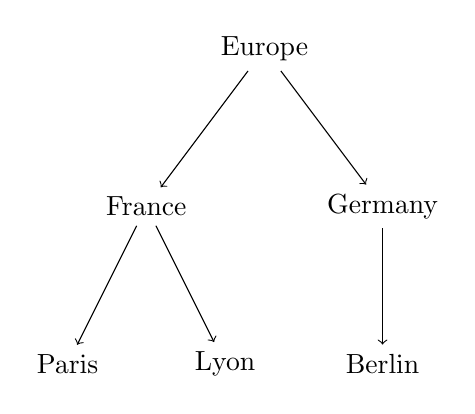
\begin{tikzpicture}
			\node[] at(1.5, 2) (E) {Europe};
			\node[] at(0, 0) (F) {France};
			\node[] at(3, 0) (G) {Germany};
			\node[] at(-1, -2) (P) {Paris};
			\node[] at(1, -2) (L) {Lyon};
			\node[] at(3, -2) (B) {Berlin};
			\draw[->] (F) -- (P);
			\draw[->] (F) -- (L);
			\draw[->] (G) -- (B);
			\draw[->] (E) -- (F);
			\draw[->] (E) -- (G);
		\end{tikzpicture}
		\caption{Hasse diagram for $\lbrace \textit{Europe}, \textit{France}, \textit{Germany}, \textit{Paris}, \textit{Lyon}, \textit{Berlin} \rbrace$}\label{fig:hasse-locations}
	\end{subfigure}
	\caption{Hasse diagrams generated by $\vDash$ on two possible sets of propositional alternatives.}\label{fig:hasse}
\end{figure}

How are these diagrams obtained from propositional alternatives, and the entailment relations between them? Formally, a Hasse diagram is a directed graph, as defined in (\ref{ex:directed-graph}). The only difference between a graph and a directed graph, is that the edges of a directed graph have a direction, i.e. they correspond to ordered pairs instead of sets of cardinality 2. If $[N_1, N_2]$ is a directed edge, $[N_1, N_2]$ is visually represented as $N_1 \rightarrow N_2$. Paths are also directed, and so is the ancestor relation (see (\ref{ex:directed-graph-path}) and (\ref{ex:directed-ancestor})). Directed graphs are designed to model \textit{asymmetric} relations, like $\vDash$.

\begin{exe}
	\ex {\textit{Directed graph.} A directed graph is defined by a set of nodes $\mathcal{N}$ and by a set of directed edges $\mathcal{E}$ between elements of $\mathcal{N}$. Directed edges are defined as ordered pairs of nodes: $\mathcal{E} \subseteq \lbrace [N_1, N_2] \ | \ (N_1, N_2) \in \mathcal{N}^2\rbrace$}\label{ex:directed-graph}
	\ex {\textit{Directed Path.} Let $G = (\mathcal{N}, \mathcal{E})$ be a directed graph. Let $(N_1, N_2) \in \mathcal{N}^2$ be two nodes of $G$. There is a path in $G$ between $N_1$ and $N_2$ (abbreviated $N_1 \stackrel{G}{\leadsto}  N_2$) iff $N_1$ can be connected to $N_2$ by a series of directed edges in $G$, i.e. $\exists (e_1, ... e_k) \in \mathcal{E}^k. \ e_1^{(0)} = N_1 \wedge e_k^{(1)} = N_2  \wedge \forall i \in [1; k-1]. \ e_i^{(1)} = e_{i+1}^{(0)}$, where, for any edge $e$,  $e = [e^{(0)}, e^{(1)}]$.}\label{ex:directed-graph-path}
	\ex {\textit{Ancestor relation (directed path version).} Let $G = (\mathcal{N}, \mathcal{E})$ be a directed graph. Let $(N_1, N_2) \in \mathcal{N}^2$. $N_1$ is an ancestor of $N_2$ iff $N_1 \stackrel{G}{\leadsto} N_2$.}\label{ex:directed-ancestor}
\end{exe}

The directed graphs (not yet the Hasse diagrams) induced by $\vDash$ on the sets of alternatives from Figure \ref{fig:hasse}, are given in Figure \ref{ex:graph-entailment}. In these graphs, there is a directed edge $[p, q]$ between two nodes corresponding to propositions $p$ and $q$, iff $p \vDash q$. Figure \ref{fig:entailment-graph-scalar} already looks like the corresponding Hasse diagram in Figure \ref{fig:hasse-scalar}, but Figure  \ref{fig:entailment-graph-locations} does not: it features a few more directed edges (in red) than its Hasse counterpart in Figure \ref{fig:hasse-locations}.

\begin{figure}[H]
	\centering
	\begin{subfigure}[t]{.45\linewidth}
		\centering
		\begin{tikzpicture}
			\node[] at(0, 0) (A) {all};
			\node[] at(0, -2) (B) {some};
			\node[] at(2, -1) (C) {none};
			\draw[->] (A) -- (B);
		\end{tikzpicture}
		\caption{Directed graph induced by $\vDash$ on $\lbrace \textit{all}, \textit{some}, \textit{none} \rbrace$}\label{fig:entailment-graph-scalar}
	\end{subfigure}	
	\hfill
	\begin{subfigure}[t]{.45\linewidth}
		\centering
		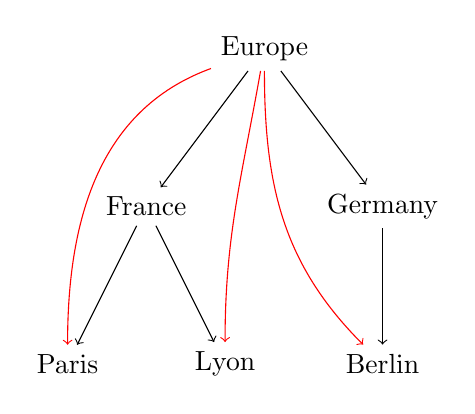
\begin{tikzpicture}
			\node[] at(1.5, 2) (E) {Europe};
			\node[] at(0, 0) (F) {France};
			\node[] at(3, 0) (G) {Germany};
			\node[] at(-1, -2) (P) {Paris};
			\node[] at(1, -2) (L) {Lyon};
			\node[] at(3, -2) (B) {Berlin};
			\draw[->] (F) -- (P);
			\draw[->] (F) -- (L);
			\draw[->] (G) -- (B);
			\draw[->] (E) -- (F);
			\draw[->] (E) -- (G);
			\draw[->,color=red] (E) to [out=-90,in=135] (B);
			\draw[->,color=red] (E) to [out=-100,in=90] (L);
			\draw[->,color=red] (E) to [out=-160,in=90] (P);
		\end{tikzpicture}
		\caption{Directed graph induced by $\vDash$ on $\lbrace \textit{Europe}, \textit{France}, \textit{Germany}, \textit{Paris}, \textit{Lyon}, \textit{Berlin} \rbrace$}\label{fig:entailment-graph-locations}
	\end{subfigure}
	\caption{Directed graphs generated by $\vDash$ on two possible sets of propositional alternatives.}\label{ex:graph-entailment}
\end{figure}

How do Hasse diagrams eliminate these few superfluous edges? The Hasse diagrams we are interested in correspond to the transitive reduction of the graphs in Figure \ref{ex:graph-entailment}, which were induced by $\vDash$ on sets of propositional alternatives. The transitive reduction operation precisely gets rid of the red edges in Figure \ref{fig:hasse-locations}, based on the idea that such edges correspond to paths formed by the black ones. The formal (though, non constructive) definition of a transitive reduction, is given in (\ref{ex:transitive-reduction}). This definition maps the graphs in Figure \ref{ex:graph-entailment}, to the Hasse diagrams in Figure \ref{fig:hasse}.

\begin{exe}
	\ex {\textit{Transitive reduction of a graph.} Let $G = (\mathcal{N}, \mathcal{E})$ be a graph. The transitive reduction $G'$ of $G$ is the graph:
	\begin{itemize}
		\item Whose set of nodes is $\mathcal{N}$;
		\item Whose edges are the smallest set $\mathcal{E'}$ s.t. $\forall (N_1, N_2) \in \mathcal{N}. \ N_1 \stackrel{G}{\leadsto} N_2 \iff N_1 \stackrel{G'}{\leadsto} N_2$
		\end{itemize}}\label{ex:transitive-reduction}
\end{exe}

The Hasse diagram in Figure \ref{fig:hasse-locations} is basically a rooted tree, and may look like a Qtree, but this is not a generality. For instance, the Hasse diagram in Figure \ref{fig:hasse-scalar} is not connected, so is not even a tree. Additionally, not all sets of propositional alternatives, even if their Hasse diagram is tree-like, are guaranteed to verify the partition property of Qtrees. The next Section focuses on how Hasse diagrams can be used to determine how alternatives relate to each other in terms of granularity. This will eventually allow us to encode granularity in the structure of Qtree.



\subsection{Alternatives and granularity}

In this section, we use a notion of granularity to constrain what kind of Qtree can be evoked by a simplex assertive LF. The goal is to organize the layers of a Qtree in terms of how specific the nodes in this layer are. Why is an external notion of granularity needed to structure Qtree? In the Qtree sketched in e.g. Figure \ref{fig2:paris-qtree}, each layer corresponds to an intuitive degree of specificity: a by-country layer dominates a by-city layer. Though intuitive, this kind of configuration is not the only one to verify the Qtree property. The tree in Figure \ref{fig2:paris-qtree-mixed}, where the \textit{Germany}-node is replaced by its children, is also a Qtree: at our level of approximation, all countries but Germany, plus all the German cities, partition the set of all possible locations, and, each country represented in this tree is properly partitioned by the set of its cities.


\begin{figure}[H]
	\centering
		\begin{forest}
			[{CS\\
				Jo grew up in...}[\textcolor{blue}{France}[\textcolor{orange}{{\fbox{Paris}}}][\textcolor{orange}{Lyon}][\textcolor{orange}{...}]][\textcolor{orange}{Berlin}][\textcolor{orange}{...}][\textcolor{blue}{Italy}[\textcolor{orange}{...}]][\textcolor{blue}{...}]]
		\end{forest}
		\caption{``Unintuitive'' Qtree for (\ref{ex2:city-partition}) = \textit{Which city did Jo grow up in?}, where layers exhibit ``mixed granularity''.}\label{fig2:paris-qtree-mixed}
	\end{figure}

To derive Qtrees like Figure \ref{fig2:paris-qtree}, and rule-out Qtrees like Figure \ref{fig2:paris-qtree-mixed}, we need a notion of granularity that can transfer into the Qtree layers. We now show that a relation of same-granularity can be derived from Hasse diagrams induced by $\vDash$ on ``complete'' sets of propositional alternatives. Considering such diagrams, where \textit{all} relevant alternatives are considered, we take that two nodes (two propositional alternatives) have same granularity if they are equidistant (in terms of path length) to a common ancestor. This relation, defined in (\ref{ex:granularity}) is close in spirit to \citet{Ippolito2019}'s \textit{Specificity Condition}.\footnote{However, the structure on which this condition operates in \citeauthor{Ippolito2019}'s model, appears slightly different (\textit{Structured Sets of Alternatives}). Also, the \textit{Specificity Condition} is not taken to be a relation, but a rather, a constraint defining which kind of alternative can be raised in e.g. disjunctive environments.} Note that this definition is conditional, and not biconditional: nodes that do not have a common ancestor, may or may not be seen as same-granularity.\footnote{This will be discussed in more detail when dealing with scalar alternatives such as $\langle$\textit{some}, \textit{all}$\rangle$, in Chapter \ref{chap:scalarity}. It will be crucial that such alternatives, which do \textit{not} have a common ancestor in their Hasse diagram (see Figure \ref{fig:hasse-scalar}), \textit{can} be seen as same-granularity.}

\begin{exe}
	\ex {\textit{Same granularity relation $\sim_g$.} Let $p$ and $q$ be two propositions belonging to the same set of propositional alternatives. Let $H$ be the Hasse diagram induced by $\vDash$ on this set of alternatives. If $p$ and $q$ have a common ancestor $r$ in $H$, and the paths from $r$ to $p$ and $r$ to $q$ have same length, then $p \sim_g q$.}\label{ex:granularity}
\end{exe}

We now leverage this relation between propositions to define the layers of a Qtree as partitions induced by sets of same-granularity alternatives. We first observe that the relation $\sim_g$ defined in (\ref{ex:granularity}) can be used to divide the set of propositional alternatives to a given LF, into subsets sharing the same level of granularity. This gives rise to a ``tiered'' set of alternatives, as defined in (\ref{ex:tiered-alternatives}). 
\begin{exe}
	\ex {\textit{Tiered set of propositional alternatives.} Let $X$ be a sentence denoting a proposition $p$. A tiered set of propositional alternatives to $X$, is the set of sets of propositions, whose elements are the maximal sets of propositions related by the same-granularity relation. In other words,  $\mathcal{A}_{p, X}^{\sim_g} = \lbrace \lbrace r \in \mathcal{A}_{p, X} \ | \ r \sim_g q \rbrace \ | \ q \in \mathcal{A}_{p, X}\rbrace$. If $\sim_g$ is an equivalence relation, $\mathcal{A}_{p, X}^{\sim_g}$ is a partition.} \label{ex:tiered-alternatives}
\end{exe}

Tiered sets of alternatives are quite close to the \textit{Structured Sets of Alternatives} defined in \citet{Ippolito2019}. One difference however, is that tiered sets of propositional alternatives are \textit{not} assumed to include propositions corresponding to alternatives that are more complex than the original LF. The elements of a tiered set of propositional alternatives are sets of propositions and form same-granularity ``tiers'', as defined in (\ref{ex:granularity-tier}). These tiers will be used to form Qtree layers. If $\sim_g$ is an equivalence relation when restricted to a specific set of propositional alternatives, then the resulting tiered set of alternatives will partition it, i.e. same-granularity tiers will be cells.

\begin{exe}
	\ex {\textit{Same-granularity tier.} Let $X$ be a sentence denoting a proposition $p$, and $\mathcal{A}_{p, X}$ its set of propositional alternatives. Let $q \in \mathcal{A}_{p, X}$. The set of same-granularity alternatives to $q$ (in $\mathcal{A}_{p, X}$), is the set of propositions in $\mathcal{A}_{p, X}$ sharing same-granularity with $q$. We call this set $\mathcal{A}^q_{p, X}$. $\mathcal{A}^q_{p, X} = \lbrace r \in \mathcal{A}_{p, X} \ | \ r \sim_g q\rbrace$. $\mathcal{A}^q_{p, X}$ is a subset of the tiered set of propositional alternatives to $X$, $\mathcal{A}_{p, X}^{\sim_g}$. Moreover, if $\sim_g$ is an equivalence relation, then $\mathcal{A}^q_{p, X}$ constitutes a cells of $\mathcal{A}_{p, X}^{\sim_g}$. }\label{ex:granularity-tier}
\end{exe}

\subsection{Leveraging alternatives to generate Qtrees}
We are now equipped to devise a recipe generating Qtrees out of simplex sentences, based on tiered sets of propositional alternatives. We start by considering the standard constraint on question-answer pairs, given in (\ref{ex:con-q-a}). This constraint establishes a connection between the standard set of alternatives derived from a sentence involving focus, and the kind of question this sentence answers.

\begin{exe}
	\ex {\textit{Constraint on question-answer pairs (\citenp{Rooth1992}, to be revised).} A good question-answer pair $(Q, A)$ is s.t. $\llbracket Q \rrbracket \subseteq \llbracket A\rrbracket^f$, where:
	\begin{itemize}
		\item $\llbracket Q \rrbracket$ corresponds to the alternative semantics of the question;
		\item $\llbracket A\rrbracket^f$ corresponds to the focus semantic value of the answer, i.e. the set of propositions denoted by LFs obtained from $A$ \textit{via} the substitution of $A$'s focused material by a same-type element.
		\end{itemize}}\label{ex:con-q-a}
\end{exe}

Let us show that this constraint is not sufficient (though, a good starter) for a model of questions evoked by assertions. We assume that $A$ corresponds to the sentence \textit{Jo grew up in PARIS}, where \textit{PARIS} is focused. The focus semantic value of $A$ then involves propositions denoted by LFs of the form \textit{Jo grew up in l}, with \textit{l} a location, e.g. \textit{Paris}, \textit{France}, or \textit{Germany}. If the only constraint on the question $Q$ accommodated from $A$ was that $\llbracket Q \rrbracket$ should be a subset of  $\llbracket A\rrbracket^f$, then, in principle, $\llbracket Q \rrbracket$ could be made of the three propositions that \textit{Jo grew up in Paris}, \textit{Jo grew up in France}, and \textit{Jo grew up in Germany}. Granted that Paris is in France, and that France and Germany are disjoint, this set of alternatives would induce a partition of the CS of the form $\lbrace \neg \textit{France} \wedge \neg \textit{Germany}, \textit{Germany}, \textit{France} \wedge \neg \textit{Paris}, \textit{Paris}\rbrace$. This appears similar to the mixed-granularity layer that we said was problematic in Figure \ref{fig2:paris-qtree-mixed}. So not all questions allowed by (\ref{ex:con-q-a}), given a fixed assertion, appear to make sense. There are two ways to alter (\ref{ex:con-q-a}) to avoid that kind of configuration: modify the relation between $\llbracket Q\rrbracket$ and $\llbracket A \rrbracket^f$, and/or, change $\llbracket A \rrbracket^f$ into something else.

We in fact opt for both options, and reuse the ideas presented in the previous Section. Specifically, we consider two subcases: the case in which $\llbracket Q \rrbracket$ simply corresponds to $\lbrace \llbracket A \rrbracket \rbrace$, and induces a partition of the CS of the form $\lbrace \llbracket A \rrbracket, \neg\llbracket A \rrbracket \rbrace$; and the case foreshadowed in the previous section, in which $\llbracket Q \rrbracket$ corresponds to same-granularity alternatives to $\llbracket A \rrbracket$. These two cases are repeated in (\ref{ex:con-q-a-gran}).

\begin{exe}
	\ex {\textit{Constraint on question-answer pairs (first revision).} Let $X$ be a LF denoting $p$. $X$ evokes a question that is either:
		\begin{enumerate}[(i)]
			\item\label{ex:con-q-a-gran-singleton} $\llbracket Q \rrbracket = \lbrace p \rbrace$;
			\item\label{ex:con-q-a-gran-tier} $\llbracket Q \rrbracket = \mathcal{A}^p_{p, X}$, the set of same-granularity alternatives to $p$.
	\end{enumerate}}\label{ex:con-q-a-gran}
\end{exe}


(\ref{ex:con-q-a-gran}) allows assertions to evoke multiple potential Qtrees. According to (\ref{ex:con-q-a-gran}), an assertion such as \textit{Jo grew up in Paris}, will either evoke the question $\llbracket Q \rrbracket = \lbrace \textit{Paris} \rbrace$, inducing a partition of the CS of the form $\lbrace \textit{Paris}, \neg\textit{Paris}\rbrace$, and corresponding to the polar question of whether or not Jo grew up in Paris; or, $\llbracket Q \rrbracket = \lbrace \textit{Paris}, \textit{Lyon}, \textit{Nice}, ..., \textit{Berlin}, ..., \textit{Rome}, ... \rbrace$, inducing a similar partition of the CS, and corresponding to the \textit{wh}-question \textit{In which city did Jo grow up?}. These partitions are represented in Figure \ref{fig:one-layer-qtrees}. 

\begin{figure}[H]
	\centering
	\begin{subfigure}[t]{.45\linewidth}
		\centering
		\begin{forest}
			[CS [\textcolor{orange}{Paris}] [\textcolor{orange}{$\neg${Paris}}]]
		\end{forest}
		\caption{A Qtree for (\ref{ex:city-assertion}) assuming (\ref{ex:con-q-a-gran}\ref{ex:con-q-a-gran-singleton}) }\label{fig:one-layer-polar}
	\end{subfigure}
	\hfill
	\begin{subfigure}[t]{.5\linewidth}
		\centering
		\begin{forest}
			[CS [\textcolor{orange}{Paris}] [\textcolor{orange}{Lyon}] [\textcolor{orange}{...}] [\textcolor{orange}{Berlin}] [\textcolor{orange}{...}] [\textcolor{orange}{Rome}]]
		\end{forest}
		\caption{A Qtree for (\ref{ex:city-assertion}) assuming (\ref{ex:con-q-a-gran}\ref{ex:con-q-a-gran-tier})}\label{fig:one-layer-wh}
	\end{subfigure}
	\caption{One-layer Qtrees generable from (\ref{ex:con-q-a-gran}) and the sentence (\ref{ex:city-assertion})=\textit{Jo grew up in Paris}.}\label{fig:one-layer-qtrees}
\end{figure}

The above partitions seem more in line with intuitions than the pathological ones generable from (\ref{ex:con-q-a}). However, they still do not form layered Qtrees. Therefore, (\ref{ex:con-q-a-gran}) is still not powerful enough to capture the specificity differences sketched in Figure \ref{fig:qtrees-diff-gran} among others. Going one step further, we can assume that the Qtrees compatible with a sentence, are either generated by the proposition $p$ denoted by the sentence (thus creating a Qtree like Figure \ref{fig:one-layer-polar}), or, by the sentence's tiered set of propositional alternatives, as defined in (\ref{ex:tiered-alternatives}). Specifically in the latter case, it will be assumed that each layer of the Qtree corresponds to the partition induced on the CS by a same-granularity tier of propositional alternatives, and that layers are ordered in terms of granularity. Figure \ref{fig:one-layer-wh} constitutes the simplest subcase of this principle, in which only one layer gets generated out of same-granularity alternatives to $p$. In any case, verifying nodes are defined as the leaves of the tree entailing $p$ (i.e. contained in $p$). This is formalized in (\ref{ex:qtree-simplex-def}). In this definition, (\ref{ex:qtree-simplex-def}\ref{pt:simplex-qtree-wh}) may be seen as a subcase of (\ref{ex:qtree-simplex-def}\ref{pt:simplex-qtree-tiered}), in which the $p$-chain set to $p$ only.

\begin{exe}
	\ex {\textit{Qtrees for simplex LFs (to be further generalized in Chapter \ref{chap:scalarity}). }
		Let $X$ be a simplex LF denoting $p$, not settled in the CS. Let $\mathcal{A}_{p, X}$ be the set $X$'s propositional alternatives. For any $q \in  \mathcal{A}_{p, X}$, let $\mathcal{A}^q_{p, X} \subseteq \mathcal{A}_{p, X}$ be the set of alternatives from $\mathcal{A}_{p, X}$ sharing same granularity with $q$. We assume for simplicity that for any $q$, $\mathcal{A}^q_{p, X}$ partitions the CS. A Qtree for $X$ is either:
		\begin{enumerate}[(i)]
			\item\label{pt:simplex-qtree-polar} A depth-1 Qtree whose leaves denote $\mathfrak{P}_{\lbrace p \rbrace, CS} = \lbrace p, \neg p\rbrace$
			\item\label{pt:simplex-qtree-wh} A depth-1 Qtree whose leaves denote $\mathfrak{P}_{\mathcal{A}^p_{p, X}, CS} = \mathcal{A}^p_{p,X}$.
			\item\label{pt:simplex-qtree-tiered} A depth-$k$ Qtree ($k > 1$) constructed in the following way:
			\begin{itemize}
				\item Formation of a ``$p$-chain'' $p_0 = p \subset p_1 \subset ... \subset p_n$ where $p_0, ...,  p_n$ are all in $\mathcal{A}_{p, X}$ but belong to different granularity tiers in $\mathcal{A}_{p, X}^{\sim_g}$:  $\mathcal{A}^{p_0}_{p, X}$ $\neq$ $\mathcal{A}^{p_1}_{p, X}$ $\neq$ ... $\neq$$\mathcal{A}^{p_n}_{p, X}$.
				\item Generation of the ``layers'' of the Qtree, based on the partitions induced by the granularity tiers corresponding to each element of the $p$-chain:\\ \begin{small}$\left\lbrace\mathfrak{P}_{\mathcal{A}^{p_i}_{p, X}, CS} \ | \ i \in [0;n]\right\rbrace$\end{small}.
				\item Determination of the edges between nodes (cells) of adjacent layers (and between the highest layer and the root), based on the subset relation.\footnote{This may not always create well-formed Qtrees. Chapter \ref{chap:scalarity} will explore such cases update (\ref{ex:qtree-simplex-def}) in consequence.}
			\end{itemize}
		\end{enumerate}
		In any case, \setlength{\fboxsep}{2pt}\fbox{verifying nodes} are defined as the set of leaves entailing $p$.
	}\label{ex:qtree-simplex-def}
\end{exe}


\subsection{Applying the recipe to two simple sentences}

We can now apply (\ref{ex:qtree-simplex-def}) to sentences like (\ref{ex:city-assertion}) and (\ref{ex:country-assertion}), repeated below.

\begin{exe}
	\exr{ex:city-country-assertions}
	\begin{xlist}
		\ex {Jo grew up in Paris.}
		\ex {Jo grew up in France.}
	\end{xlist}
\end{exe}

We start with (\ref{ex:city-assertion}), and assume that its alternatives are of the form \textit{Jo grew up in l}, with \textit{l} a city or a country. Taking for granted that ``city'' propositions and ``country'' propositions form two distinct granularity tiers, the tiered set of propositional alternatives to (\ref{ex:city-assertion}), will be as in (\ref{ex:city-tiered-alt}).

\begin{exe}
	\ex {$\mathcal{A}_{\textit{Paris}, (\ref{ex:city-assertion})}^{\sim_g} = \lbrace \lbrace \textit{Paris}, \textit{Lyon}, ..., \textit{Berlin}, ...\rbrace, \lbrace\textit{France}, \textit{Germany}, ...\rbrace\rbrace$\\
	\phantom{$\mathcal{A}_{\textit{Paris}, (\ref{ex:city-assertion})}^{\sim_g}$} $=\lbrace\lbrace p \ | \ \exists l. \ \text{$l$ is a city} \wedge \ p = \lambda w. \ \text{Jo grew up in $l$ in $w$}\rbrace,$\\
	\phantom{$\mathcal{A}_{\textit{Paris}, (\ref{ex:city-assertion})}^{\sim_g} = \lbrace$}$\lbrace p \ | \ \exists l. \ \text{$l$ is a country} \wedge \ p = \lambda w. \ \text{Jo grew up in $l$ in $w$}\rbrace\rbrace$}\label{ex:city-tiered-alt}
\end{exe} 



First, we can generate a Qtree for (\ref{ex:city-assertion})  using principle (\ref{ex:qtree-simplex-def}\ref{pt:simplex-qtree-polar}). This Qtree will have the CS as root, and two leaves corresponding to the propositions that \textit{Jo grew up in Paris}, and \textit{Jo did not grow up in Paris} (assuming this matter is not settled in the CS). This Qtree is depicted in Figure \ref{fig:city-qtree-polar}. Intuitively, it corresponds to the question of whether or not Jo grew up in Paris.

Second, we can use principle (\ref{ex:qtree-simplex-def}\ref{pt:simplex-qtree-wh}). To do so, we must determine the set of same-granularity alternatives to the prejacent proposition that \textit{Jo grew up in Paris}. This set, labeled $\mathcal{A}_{\textit{Paris}, (\ref{ex:city-assertion})}^{\textit{Paris}}$, corresponds to the first element of the tiered set of propositional alternatives $\mathcal{A}_{\textit{Paris}, (\ref{ex:city-assertion})}^{\sim_g}$ in  (\ref{ex:city-tiered-alt}). It is repeated in (\ref{ex:city-gran-alt}). The alternatives contained in $\mathcal{A}_{\textit{Paris}, (\ref{ex:city-assertion})}^{\textit{Paris}}$ are all exclusive (cities are spatially disjoint), and moreover cover the space of possibilities. So, once intersected with the CS, they already form a partition of the CS. According to principle (\ref{ex:qtree-simplex-def}\ref{pt:simplex-qtree-wh}), this partition correspond to the leaves of the resulting Qtree. This Qtree is depicted in Figure \ref{fig:city-qtree-wh}. Intuitively, it corresponds to the question of which city Jo grew up in.


\begin{exe}
	\ex {$\mathcal{A}_{\textit{Paris}, (\ref{ex:city-assertion})}^{\textit{Paris}} = \lbrace \textit{Paris}, \textit{Lyon}, ..., \textit{Berlin}, ...\rbrace$\\
		\phantom{$\mathcal{A}_{\textit{Paris}, (\ref{ex:city-assertion})}^{\sim_g}$} $=\lbrace p \ | \ \exists l. \ \text{$l$ is a city} \wedge \ p = \lambda w. \ \text{Jo grew up in $l$ in $w$}\rbrace$\\
		\phantom{$\mathcal{A}_{\textit{Paris}, (\ref{ex:city-assertion})}^{\sim_g}$} $=\mathfrak{P}_{\lbrace \textit{Paris}, \textit{Lyon}, ..., \textit{Berlin}, ...\rbrace, CS}$}\label{ex:city-gran-alt}
\end{exe} 

Third and lastly, we can use principle (\ref{ex:qtree-simplex-def}\ref{pt:simplex-qtree-tiered}), which constitutes are multi-layer generalization of principle (\ref{ex:qtree-simplex-def}\ref{pt:simplex-qtree-wh}). To do so, we need to define a $p$-chain of propositions entailed $p$ = $\lambda w. \ $\textit{Jo grew up in Paris in $w$}. The tiered set of alternatives posited in (\ref{ex:city-tiered-alt}) contains one such proposition, namely $p' = \lambda w. \ $\textit{Jo grew up in France in $w$}. The resulting Qtree will therefore be made of three layers: the CS (root), the partition generated by the same granularity alternatives to $p'$, and the partition generated by the same granularity alternatives to $p$, already defined in (\ref{ex:city-gran-alt}). The set of same-granularity alternatives to $p'$, labeled $\mathcal{A}_{\textit{Paris}, (\ref{ex:city-assertion})}^{\textit{France}}$, corresponds to the second element of the tiered set of propositional alternatives $\mathcal{A}_{\textit{Paris}, (\ref{ex:city-assertion})}^{\sim_g}$ in  (\ref{ex:city-tiered-alt}). It is repeated in (\ref{ex:country-gran-alt}). The alternatives contained in $\mathcal{A}_{\textit{Paris}, (\ref{ex:city-assertion})}^{\textit{France}}$ are all exclusive (country are spatially disjoint), and moreover cover the space of possibilities. So, once intersected with the CS, they already form a partition of the CS. 

\begin{exe}
	\ex {$\mathcal{A}_{\textit{Paris}, (\ref{ex:city-assertion})}^{\textit{France}} = \lbrace \textit{France}, \textit{Germany}, ...\rbrace$\\
		\phantom{$\mathcal{A}_{\textit{Paris}, (\ref{ex:city-assertion})}^{\sim_g}$} $=\lbrace p \ | \ \exists l. \ \text{$l$ is a country} \wedge \ p = \lambda w. \ \text{Jo grew up in $l$ in $w$}\rbrace$\\
		\phantom{$\mathcal{A}_{\textit{Paris}, (\ref{ex:city-assertion})}^{\sim_g}$} $=\mathfrak{P}_{\lbrace \textit{France}, \textit{Germany}, ...\rbrace, CS}$}\label{ex:country-gran-alt}
\end{exe} 

As per principle (\ref{ex:qtree-simplex-def}\ref{pt:simplex-qtree-tiered}), a Qtree evoked by (\ref{ex:city-assertion}) will then have the CS as top layer, the nodes corresponding to the partition in (\ref{ex:country-gran-alt}) as middle layer, and the nodes corresponding to the partition in (\ref{ex:city-gran-alt}) as bottom (leaf) layer. Connectivity between layers is straightforward: it corresponds to the inclusion relation between cities and countries, and between countries and ``the whole world'' ($\sim$CS). The resulting Qtree is given in Figure \ref{fig:city-qtree-tiered}. Intuitively, it corresponds to the question of which city Jo grew up in, but such that this question is decomposed into two subquestions: first, which country Jo grew up in; then, knowing the country, which city Jo grew up in, in that country.


\begin{figure}[H]
	\centering
	\begin{subfigure}[t]{.23\linewidth}
		\centering
		\scalebox{.85}{
		\begin{forest}
			[CS [\textcolor{orange}{\fbox{Paris}}] [\textcolor{orange}{$\neg$Paris}]]
		\end{forest}}
		\caption{Following principle (\ref{ex:qtree-simplex-def}\ref{pt:simplex-qtree-polar}).}\label{fig:city-qtree-polar}
	\end{subfigure}
	\hfill
	\begin{subfigure}[t]{.33\linewidth}
		\centering		\scalebox{.85}{
		\begin{forest}
			[CS [\textcolor{orange}{\fbox{Paris}}] [\textcolor{orange}{Lyon}] [\textcolor{orange}{...}][\textcolor{orange}{Berlin}][\textcolor{orange}{...}]]
		\end{forest}}
		\caption{Following principle (\ref{ex:qtree-simplex-def}\ref{pt:simplex-qtree-wh}).}\label{fig:city-qtree-wh}
	\end{subfigure}
	\hfill
	\begin{subfigure}[t]{.38\linewidth}
		\centering\scalebox{.85}{
		\begin{forest}
			[CS [\textcolor{blue}{France}[\textcolor{orange}{\fbox{Paris}}] [\textcolor{orange}{Lyon}] [\textcolor{orange}{...}]] [\textcolor{blue}{Germany}[\textcolor{orange}{Berlin}][\textcolor{orange}{...}]][\textcolor{blue}{...}]]
		\end{forest}}
		\caption{Following principle (\ref{ex:qtree-simplex-def}\ref{pt:simplex-qtree-tiered}).}\label{fig:city-qtree-tiered}
	\end{subfigure}
	\caption{Possible Qtrees evoked by the assertion (\ref{ex:city-assertion})=\textit{Jo grew up in Paris}.}\label{fig:city-qtrees}
\end{figure}

Of course, if more alternatives to (\ref{ex:city-assertion}) had been posited in the first place, principle (\ref{ex:qtree-simplex-def}\ref{pt:simplex-qtree-tiered}) would have produced more Qtrees. For instance, if continent alternative had been considered, the tiered set of propositional alternatives to (\ref{ex:city-assertion}), $\mathcal{A}_{\textit{Paris}, (\ref{ex:city-assertion})}^{\sim_g}$, would have been as in (\ref{ex:city-tiered-alt-plus-continent}), and the Qtrees generated by principle (\ref{ex:qtree-simplex-def}\ref{pt:simplex-qtree-tiered}), would have been the one in Figure \ref{fig:city-qtree-tiered}, plus the one in Figure \ref{fig:city-qtree-tiered-plus-continent}.

\begin{exe}
	\ex {$\mathcal{A}_{\textit{Paris}, (\ref{ex:city-assertion})}^{\sim_g} = \lbrace \lbrace \textit{Paris}, \textit{Lyon}, ..., \textit{Berlin}, ...\rbrace, \lbrace\textit{France}, \textit{Germany}, ...\rbrace, \lbrace \textit{Europe}, \textit{Asia}, ...\rbrace\rbrace$\\
		\phantom{$\mathcal{A}_{\textit{Paris}, (\ref{ex:city-assertion})}^{\sim_g}$} $=\lbrace\lbrace p \ | \ \exists l. \ \text{$l$ is a city} \wedge \ p = \lambda w. \ \text{Jo grew up in $l$ in $w$}\rbrace,$\\
		\phantom{$\mathcal{A}_{\textit{Paris}, (\ref{ex:city-assertion})}^{\sim_g} = \lbrace$}$\lbrace p \ | \ \exists l. \ \text{$l$ is a country} \wedge \ p = \lambda w. \ \text{Jo grew up in $l$ in $w$}\rbrace$\\
		\phantom{$\mathcal{A}_{\textit{Paris}, (\ref{ex:city-assertion})}^{\sim_g} = \lbrace$}$\lbrace p \ | \ \exists l. \ \text{$l$ is a continent} \wedge \ p = \lambda w. \ \text{Jo grew up in $l$ in $w$}\rbrace\rbrace$}\label{ex:city-tiered-alt-plus-continent}
\end{exe} 

\begin{figure}[H]
	\centering
	\scalebox{.85}{
		\begin{forest}
			[CS [Europe [\textcolor{blue}{France}[\textcolor{orange}{\fbox{Paris}}] [\textcolor{orange}{Lyon}] [\textcolor{orange}{...}]] [\textcolor{blue}{Germany}[\textcolor{orange}{Berlin}][\textcolor{orange}{...}]][\textcolor{blue}{...}]][Asia [...]][...] ]
	\end{forest}}
	\caption{An extra Qtree for (\ref{ex:city-assertion}), generated by principle (\ref{ex:qtree-simplex-def}\ref{pt:simplex-qtree-tiered}), assuming that (\ref{ex:city-assertion})'s tiered set of propositional alternatives is as in (\ref{ex:city-tiered-alt-plus-continent}). .}\label{fig:city-qtree-tiered-plus-continent}
\end{figure}

For simplicity and ease of comparison, we will stick to a tiered set of alternatives involving city- and country-tiers, as defined in (\ref{ex:city-tiered-alt}). Similarly, we can derive Qtrees for (\ref{ex:country-assertion})=\textit{Jo grew up in France}. This assertion will in fact require less work, because it appears coarser-grained than (\ref{ex:city-assertion}). To ensure that (\ref{ex:city-assertion}) and (\ref{ex:country-assertion}) are analyzed at the same level of approximation, we assume that (\ref{ex:country-assertion})'s alternatives are also of the form \textit{Jo grew up in l}, with \textit{l} a city or a country. The tiered set of propositional alternatives to (\ref{ex:country-assertion}) is therefore identical to that of (\ref{ex:city-assertion}), and given in (\ref{ex:country-tiered-alt}).

\begin{exe}
	\ex {$\mathcal{A}_{\textit{France}, (\ref{ex:country-assertion})}^{\sim_g} = \lbrace \lbrace \textit{Paris}, \textit{Lyon}, ..., \textit{Berlin}, ...\rbrace, \lbrace\textit{France}, \textit{Germany}, ...\rbrace\rbrace$\\
		\phantom{$\mathcal{A}_{\textit{France}, (\ref{ex:country-assertion})}^{\sim_g}$} $=\lbrace\lbrace p \ | \ \exists l. \ \text{$l$ is a city} \wedge \ p = \lambda w. \ \text{Jo grew up in $l$ in $w$}\rbrace,$\\
		\phantom{$\mathcal{A}_{\textit{France}, (\ref{ex:country-assertion})}^{\sim_g} = \lbrace$}$\lbrace p \ | \ \exists l. \ \text{$l$ is a country} \wedge \ p = \lambda w. \ \text{Jo grew up in $l$ in $w$}\rbrace\rbrace$\\
		\phantom{$\mathcal{A}_{\textit{France}, (\ref{ex:country-assertion})}^{\sim_g}$}= $\mathcal{A}_{\textit{Paris}, (\ref{ex:city-assertion})}^{\sim_g}$}\label{ex:country-tiered-alt}
\end{exe} 


First, we can generate a Qtree for (\ref{ex:country-assertion}) using principle (\ref{ex:qtree-simplex-def}\ref{pt:simplex-qtree-polar}). This Qtree will have the CS as root, and two leaves corresponding to the propositions that \textit{Jo grew up in France}, and \textit{Jo did not grow up in France} (assuming this matter is not settled in the CS). This Qtree is depicted in Figure \ref{fig:country-qtree-polar}. Intuitively, it corresponds to the question of whether or not Jo grew up in France.

Second, we can use principle (\ref{ex:qtree-simplex-def}\ref{pt:simplex-qtree-wh}). To do so, we must determine the set of same-granularity alternatives to the prejacent proposition that \textit{Jo grew up in France}. This set, labeled $\mathcal{A}_{\textit{France}, (\ref{ex:country-assertion})}^{\textit{France}}$, corresponds to the second element of the tiered set of propositional alternatives $\mathcal{A}_{\textit{France}, (\ref{ex:country-assertion})}^{\sim_g}$. It is repeated in (\ref{ex:country-gran-alt2}). This set is also equal to the set of same-granularity alternative to \textit{France}, when the prejacent was \textit{Paris} (see (\ref{ex:country-gran-alt})). Thus, the alternatives in this set, once intersected with the CS, already form a partition of the CS. According to principle (\ref{ex:qtree-simplex-def}\ref{pt:simplex-qtree-wh}), this partition correspond to the leaves of the resulting Qtree. This Qtree is depicted in Figure \ref{fig:country-qtree-wh}. Intuitively, it corresponds to the question of which country Jo grew up in.


\begin{exe}
	\ex {$\mathcal{A}_{\textit{France}, (\ref{ex:country-assertion})}^{\textit{France}} = \lbrace \textit{France}, \textit{Germany}, ...\rbrace$\\
		\phantom{$\mathcal{A}_{\textit{France}, (\ref{ex:country-assertion})}^{\textit{France}}$} $=\lbrace p \ | \ \exists l. \ \text{$l$ is a city} \wedge \ p = \lambda w. \ \text{Jo grew up in $l$ in $w$}\rbrace$\\
		\phantom{$\mathcal{A}_{\textit{France}, (\ref{ex:country-assertion})}^{\textit{France}}$} $=\mathfrak{P}_{\lbrace \textit{France}, \textit{Germany}, ...\rbrace, CS}$\\
		\phantom{$\mathcal{A}_{\textit{France}, (\ref{ex:country-assertion})}^{\textit{France}}$} $=\mathcal{A}_{\textit{Paris}, (\ref{ex:city-assertion})}^{\textit{France}}$}\label{ex:country-gran-alt2}
\end{exe} 

Third and lastly, we could use principle (\ref{ex:qtree-simplex-def}\ref{pt:simplex-qtree-tiered}), but this principle would in fact give us nothing more than principle (\ref{ex:qtree-simplex-def}\ref{pt:simplex-qtree-wh}), given our assumptions about (\ref{ex:country-assertion})'s tiered set of propositional alternatives. This is because no proposition in $\mathcal{A}_{\textit{France}, (\ref{ex:country-assertion})}^{\sim_g}$ is weaker than $p$=\textit{$\lambda w. \ \textit{Jo grew up in France in $w$}$}, and therefore, the only $p$-chain available in the case of (\ref{ex:country-assertion}), is made of simply $p$. This $p$-chain would generate one single country-layer beyond the CS root, and the resulting Qtree, would simply be the one in Figure \ref{fig:country-qtree-wh}.\footnote{Of course, if we had considered continent-level alternatives as well, principle (\ref{ex:qtree-simplex-def}\ref{pt:simplex-qtree-tiered}) would have generated an extra Qtree for (\ref{ex:country-assertion}), characterized by a continent-layer on top of a country-layer. But this would have led us to do the same move for (\ref{ex:city-assertion}), and thus to generate the Qtree in Figure \ref{fig:city-qtree-tiered-plus-continent} for that sentence.}

\begin{figure}[H]
	\centering
	\begin{subfigure}[t]{.45\linewidth}
		\centering
		\scalebox{.85}{
			\begin{forest}
				[CS [\textcolor{blue}{\fbox{France}}] [\textcolor{blue}{$\neg$France}]]
		\end{forest}}
		\caption{Following principle (\ref{ex:qtree-simplex-def}\ref{pt:simplex-qtree-polar}).}\label{fig:country-qtree-polar}
	\end{subfigure}
	\hfill
	\begin{subfigure}[t]{.45\linewidth}
		\centering		\scalebox{.85}{
			\begin{forest}
				[CS [\textcolor{blue}{\fbox{France}}] [\textcolor{blue}{Germany}][\textcolor{blue}{...}]]
		\end{forest}}
		\caption{Following principle (\ref{ex:qtree-simplex-def}\ref{pt:simplex-qtree-wh}).}\label{fig:country-qtree-wh}
	\end{subfigure}
	\caption{Possible Qtrees evoked by the assertion (\ref{ex:country-assertion})=\textit{Jo grew up in France}.}
\end{figure}


Before moving on to ``compositional'' Qtrees, let us take stock.

First, the recipe in (\ref{ex:qtree-simplex-def}) defines way to determine which parse of the CS assertive sentences evoke. We have discussed in Chapter \ref{chap:introduction} that questions typically correspond to partitions of the CS \textit{in the pragmatic domain}. Semantically, questions are taken to be sets of alternatives. In that sense, Qtrees evoked by sentences should be understood as a form of ``inquisitive pragmatics'' rather than ``inquisitive semantics''. Tiered sets of propositional alternatives may be closer to the latter concept.

Second, the recipe in (\ref{ex:qtree-simplex-def}) typically generates \textit{multiple} Qtrees out of one assertion. Under our current assumptions,  (\ref{ex:city-assertion}) gives rise to three possible Qtrees, and (\ref{ex:country-assertion}), to two. So there is some degree of uncertainty about which Qtree any given sentence actually answers. Very roughly, evoked Qtrees can be ``polar'' (principle (\ref{ex:qtree-simplex-def}\ref{pt:simplex-qtree-polar})), ``\textit{wh}'' (principle (\ref{ex:qtree-simplex-def}\ref{pt:simplex-qtree-wh})), or ``\textit{wh}-articulated'' (principle (\ref{ex:qtree-simplex-def}\ref{pt:simplex-qtree-tiered})). This optionality contrasts with frameworks like inquisitive semantics, in which any given sentence is mapped to a single nonempty downward-closed set of propositions. Given this, our recipe generates more Qtrees than intuitively assumed in the previous Sections.  Additionally, this leads us to define the oddness of a sentence as equivalent to the oddness of \textit{all} sentence-Qtree pairs to sentences can generate. This was already defined in (\ref{ex2:oddness-tree-sentence}) and (\ref{ex2:oddness-sentence}), both repeated below.

\begin{exe}
	\exr{ex2:oddness-tree-sentence} {\textit{Oddness of a Qtree, given a sentence.} If a sentence $S$ evokes a Qtree $T$ and the pair ($S$, $T$) induces a vacuous labeling of verifying nodes, or violates other sentence-Qtree well-formedness constraints (tbd), then $T$ is deemed odd given $S$.}
	\exr{ex2:oddness-sentence} {\textit{Oddness of a sentence.} A sentence $S$ is odd if any Qtree $T$ it evokes is odd given $S$.}
\end{exe}


Third, we mentioned that (\ref{ex:city-assertion}) and (\ref{ex:country-assertion}), beyond the fact that they are obviously in a relation of logical entailment, are such that (\ref{ex:city-assertion}) feels more ``fine-grained'' than (\ref{ex:country-assertion}). This is somehow cashed out by the kind of Qtrees these sentences evoke. Specifically, we observe that some Qtrees (\ref{ex:city-assertion}) evokes (Figure \ref{fig:city-qtree-tiered}) constitute refinements of some Qtree (\ref{ex:country-assertion}) evokes (Figure \ref{fig:country-qtree-wh}), where refinement is defined as in (\ref{ex:qtree-refinement}), repeated below. This implication does not hold in the opposite direction: no Qtree (\ref{ex:country-assertion}) evokes, constitutes a refinement of a Qtree (\ref{ex:city-assertion}) evokes. So (in a very weak sense) finer-grained assertions evoke finer-grained Qtrees. This observation will be crucial in Chapter \ref{chap:hurford-sentences}.

\begin{exe}
	\exr{ex:qtree-refinement} {\textit{Qtree refinement.} Let $T$ and $T'$ be Qtrees. $T$ is a refinement of $T'$ (or: $T$ is finer-grained than $T'$), iff $T'$ can be obtained from $T$ by removing a subset $\mathcal{T}$ of $T$'s subtrees, s.t.:
		\begin{itemize}
			\item if $\mathcal{T}$ contains a subtree rooted in $N$, then, for each node $N'$ that is a sibling of $N$ in $T$, the subtree of $T$ rooted in $N'$, is also in $\mathcal{T}$.
	\end{itemize}}
\end{exe}

We now proceed to define Qtree for complex sentences belonging to the $\lbrace \neg, \vee, \rightarrow\rbrace$-fragment of the language. We will do so inductively, using our recipe for simplex sentences (\ref{ex:qtree-simplex-def}) as base case, along with specific combination rules corresponding to the inquisitive effect of each operator.


\section{Compositional Qtrees: inductive step}

In the previous Section, we have seen how to derive Qtrees from simplex sentences, containing no operator or connective. In this Section, we clarify how complex sentences, that may be equally informative, and may even have same propositional meaning, may end up packaging information differently from one another, in terms of their evoked Qtrees. This difference in information packaging, will allow us to derive different felicity profiles for these sentences. We start with Qtrees evoked by negated LFs, before moving on to Qtrees evoked by disjunctions and conditionals.

\subsection{Questions evoked by negated LFs}\label{sec:neg}
We assume negated LFs evoke questions that are structurally similar to those evoked by their non-negated counterpart. The only difference resides in the set of verifying nodes, which is ``flipped'' by negation. This is formalized in (\ref{ex2:qtree-neg-def}).\footnote{This approach is perhaps a bit naive; uttering $p$ vs. $\neg p$, does not seem to preferentially answer the same kind of question. More specifically, it seems that uttering negative statements in general conveys the idea that the original question was more likely to be a polar question of the form \textit{whether p?}--as opposed to a \textit{wh} kind of question. We discuss this more in depth in Chapter \ref{chap:scalarity}.}

\begin{exe}
	\ex {\textit{Qtrees for negated LFs.} Let $T$ be a Qtree evoked by a LF $X$. A Qtree $T_{\neg}$ for $\neg X$ is obtained from $T$ by:
		\begin{itemize}
			\item retaining $T$'s structure; i.e. if $T = (\mathcal{N}, \mathcal{E}, R)$,  then $T_{\neg} = (\mathcal{N}, \mathcal{E}, R)$, too;
			\item defining $T_{\neg}$'s set of verifying nodes $\mathcal{N}^+(T_{\neg})$ as the set of $T_{\neg}$'s nodes $N$ that are not verifying in $T$ ($N \notin \mathcal{N}^+(T)$) but belong to a layer containing at least one verifying node $N'$ in $T$ ($N' \in \mathcal{N}^+(T)$). In other words:\\
			$\mathcal{N}^+(T_\neg)$ = $\lbrace N \ | \ N \notin \mathcal{N}^+(T) \wedge \exists N' \in \mathcal{N}^+(T). \ d(N, T_\neg)=d(N', T_\neg) \rbrace$\\
			With $d(N, T)$ the depth of a node $N$ in a tree $T$ (see (\ref{ex:tree-depth})).\footnote{Because $T$ and $T_\neg$ have same structure, it does not matter which Qtree among $T$ and $T_\neg$ is passed as argument to the depth function; in that particular case, $\forall N \in \mathcal{N}. \ d(N, T)=d(N, T_\neg)$.}
		\end{itemize} 
	}\label{ex2:qtree-neg-def}
\end{exe}

The recipe in (\ref{ex2:qtree-neg-def}) is exemplified in the abstract Qtrees in Figure \ref{fig:qtree-x-neg-x}. 

\begin{figure}[H]
	\centering
	\begin{subfigure}[t]{.45\linewidth}
		\centering
		\begin{forest}
			[A[\fbox{B}[\fbox{E}][\fbox{F}]][C][\fbox{D}[G][H[J][K]][I]]]
		\end{forest}
		\caption{An abstract Qtree for $X$}\label{fig:qtree-x}
	\end{subfigure}
	\hfill
	\begin{subfigure}[t]{.45\linewidth}
		\centering
		\begin{forest}
			[A[{B}[{E}][{F}]][\fbox{C}][{D}[\fbox{G}][\fbox{H}[J][K]][\fbox{I}]]]
		\end{forest}
		\caption{An abstract Qtree for $\neg X$, derived from Figure \ref{fig:qtree-x}.}\label{fig:qtree-neg-x}
	\end{subfigure}
	\caption{An abstract Qtree for $X$ and the abstract Qtree for $\neg X$ derived from it, \textit{via} (\ref{ex2:qtree-neg-def}).}\label{fig:qtree-x-neg-x}
\end{figure}


It may not seem obvious at this point why and how verifying nodes would occur at intermediate levels in a Qtree; after all, all the Qtrees we have seen so far (derived from simplex sentences) had their verifying nodes at the leaf level. But we will see that Qtrees derived from complex sentences (typically, involving disjunctions and conditionals) can in principle feature intermediate verifying nodes, because such nodes are also derived compositionally.
Now, granted that verifying nodes may indeed occur at different levels, the intuition behind the ``flipping'' algorithm in (\ref{ex2:qtree-neg-def}) is the following. If a node $N$ is verifying in a Qtree $T$ corresponding to an LF $X$, and $N$ is located at depth $k$ in $T$, then somehow the $k$-layer of $T$ is ``addressed'' by $X$. We aim for a pair $(\neg X, T_\neg)$ to address the same layers as $(X, T)$, so $T_\neg$'s verifying nodes should have similar a similar depth distribution as $T$'s verifying nodes. But of course, the two sets of nodes need to be distinct, because negation standardly flips truth values--hence the by-layer flipping.

It is additionally worth mentioning that, if all verifying nodes in the original Qtree $T$ are leaves, (\ref{ex2:qtree-neg-def}) is simplified: $T_\neg$'s set of verifying nodes is simply the set of leaves in $T$/$T_\neg$ that are not verifying in $T$. This is summarized in (\ref{ex2:qtree-neg-def-leaves}).

\begin{exe}
	\ex {\textit{Qtrees for negated LFs (leaf-only version, subcase of (\ref{ex2:qtree-neg-def})).} Let $T$ be a Qtree evoked by a LF $X$ s.t. $\mathcal{N}^+(T) \subseteq \mathcal{L}(T)$, where $\mathcal{L}(T)$ refers to $T$'s leaves. A Qtree $T_{\neg}$ for $\neg X$ is obtained from $T$ by:
		\begin{itemize}
			\item retaining $T$'s structure;
			\item defining $T_{\neg}$'s set of verifying nodes as the complement set of $\mathcal{N}^+(T)$ within $\mathcal{L}(T)$:
			$\mathcal{N}^+(T_\neg) = \lbrace N \in \mathcal{L}(T)\ | \ N \notin \mathcal{N}^+(T)\rbrace$ 
		\end{itemize} 
	}\label{ex2:qtree-neg-def-leaves}
\end{exe}

Following this simplified recipe, Qtrees for (\ref{ex:city-neg-assertion}), which correspond to the negation of (\ref{ex:city-assertion}), are given below. They are obtained from Figure \ref{fig:city-qtrees}, by simply flipping boxed nodes at the leaf level. These new Qtree capture the intuition that (\ref{ex:city-neg-assertion}) can answer three kinds of question: a question about whether or not Jo grew up in Paris; a question about which city Jo grew up in; and a question about which city Jo grew up in question of which city Jo grew up in, but such that this question is decomposed into two subquestions: first, which country Jo grew up in; then, knowing the country, which city Jo grew up in, in that country. The nodes that get flagged as verifying, correspond to sets of worlds disjoint from $\lambda w. \ \textit{Jo grew up in Paris in $w$}.$ Interestingly, negation preserves Qtree granularity, simply because it preserves Qtree structure.

\begin{exe}
	\exr{ex:city-assertion} {Jo grew up in Paris.}
	\ex {Jo did not grow up in Paris.}\label{ex:city-neg-assertion}
\end{exe}


\begin{figure}[H]
	\centering
	\begin{subfigure}[t]{.23\linewidth}
		\centering
		\scalebox{.85}{
			\begin{forest}
				[CS [\textcolor{orange}{{Paris}}] [\textcolor{orange}{\fbox{$\neg$Paris}}]]
		\end{forest}}
		\caption{Following principle (\ref{ex:qtree-simplex-def}\ref{pt:simplex-qtree-polar}).}\label{fig:neg-city-qtree-polar}
	\end{subfigure}
	\hfill
	\begin{subfigure}[t]{.33\linewidth}
		\centering		\scalebox{.85}{
			\begin{forest}
				[CS [\textcolor{orange}{{Paris}}] [\textcolor{orange}{\fbox{Lyon}}] [\textcolor{orange}{\fbox{...}}][\textcolor{orange}{\fbox{Berlin}}][\textcolor{orange}{\fbox{...}}]]
		\end{forest}}
		\caption{Following principle (\ref{ex:qtree-simplex-def}\ref{pt:simplex-qtree-wh}).}\label{fig:neg-city-qtree-wh}
	\end{subfigure}
	\hfill
	\begin{subfigure}[t]{.38\linewidth}
		\centering\scalebox{.85}{
			\begin{forest}
				[CS [\textcolor{blue}{France}[\textcolor{orange}{{Paris}}] [\textcolor{orange}{\fbox{Lyon}}] [\textcolor{orange}{\fbox{...}}]] [\textcolor{blue}{Germany}[\textcolor{orange}{\fbox{Berlin}}][\textcolor{orange}{\fbox{...}}]][\textcolor{blue}{...}]]
		\end{forest}}
		\caption{Following principle (\ref{ex:qtree-simplex-def}\ref{pt:simplex-qtree-tiered}).}\label{fig:neg-city-qtree-tiered}
	\end{subfigure}
	\caption{Possible Qtrees evoked by the assertion (\ref{ex:city-neg-assertion})=\textit{Jo did not grow up in Paris}.}\label{fig:neg-city-qtrees}
\end{figure}


\subsection{Questions evoked by disjunctive LFs}

Let us consider the disjunction in (\ref{ex:city-disjunction}). Intuitively, this sentence is a good, non-maximal answer to a question like (\ref{ex2:city-question}), repeated below. It identifies two cities in which Jo could have grown up, and conveys ignorance about which city Jo actually grew up in. Note that either disjunct taken in isolation, \textit{Jo grew up in Paris}, or \textit{Jo grew up in Lyon}, constitutes a \textit{maximal} answer to (\ref{ex2:city-question}).

\begin{exe}
	\exr{ex2:city-question} {In which city did Jo grow up?}
	\ex {Jo grew up in Paris or Lyon.}\label{ex:city-disjunction}
\end{exe}

This observation is consistent with the idea that, in a felicitous disjunction, both disjuncts must answer the same kind of question \citep{Simons2001,Zhang2022}. Ou rephrasing of this observation is spelled out in (\ref{ex:disjunction-same-q}). 

\begin{exe}
	\ex {\textit{Disjunctive answer.} Let $X = Y \vee Z$ be a disjunctive LF. If $X$ is a felicitous assertion, then the set of questions $Y$ answers is equal to the set of questions $Z$ answers. Additionally, if $Y$/$Z$ answer a question, then $X$ answers it too.}\label{ex:disjunction-same-q}
\end{exe}


A way to further specify this intuition in our model, is to assume that a Qtree for $X = Y \vee Z$, must contain a Qtree for $Y$ and a Qtree for $Z$. Containment is understood as the subgraph relation (defined in (\ref{ex:subgraph})). This ensures that any node in $Y$'s Qtree is also in $X$'s Qtree, and any node in $Z$'s Qtree, is also in $X$'s Qtree. So, whatever answers $Y$ or $Z$, also answers $X$. This is modeled by assuming that the Qtrees evoked by a disjunction are all the possible well-formed unions of Qtrees evoked by each disjunct. This is spelled out in (\ref{ex2:disj-qtree}). In this definition, Qtree union builds on the notion of graph-union, as formalized in (\ref{ex:graph-union}).\footnote{I thank Amir who helped me see this.} On top of this, Qtree union involves the union of verifying nodes, and the determination of a root node for the output Qtree, defined as the maximum between the two roots of the input Qtrees.


\begin{exe}
	\ex {\textit{Qtrees for disjunctive LFs.} A Qtree $T_{\vee}$ for $X \vee Y$, if defined, is obtained from a Qtree $T_X$ for $X$ and a Qtree $T_Y$ for $Y$ by:
		\begin{itemize}
			\item graph-unioning $T_X$ and $T_Y$;
			\item defining $T_{\vee}$'s root as the maximal element (i.e. the weaker proposition) between the root of $T_X$ and the root of $T_Y$. This will typically be the entire CS. If there is no such maximum, then the output cannot be a Qtree. \footnote{Indeed, suppose $R_X$ and $R_Y$ are the roots of respectively $T_X$ and $T_Y$, and that $R_X$ and $R_Y$ are not in any kind of inclusion relation. We show by contradiction that $T_X \cup T_Y$ cannot be a Qtree. If $T_X \cup T_Y$ were a Qtree, then, $R_X$ and $R_Y$ would not be in an ancestry relation, meaning, $R_X$ would not be an ancestor of $R_Y$, and $R_Y$ would not be an ancestor of $R_X$. So, neither $R_X$ nor $R_Y$ could be the root of $T_X \cup T_Y$, because the root is an ancestor of all the other nodes. Let's call $R$ this root. $R$ is a common ancestor of both $R_X$ and $R_Y$ in $T_X \cup T_Y$. So $R$ must be a strict superset of $R_X$ and $R_Y$. Also, because $T_X \cup T_Y$ is obtained \textit{via} node- and edge-union, we must have, in the input Qtrees: $R_X \stackrel{T_X}{\leadsto} R$ and $R_Y \stackrel{T_Y}{\leadsto} R$. In other words, $R_X$ is an ancestor of $R$ in $T_X$, and $R_Y$ is an ancestor of $R$ in $T_Y$. Because $T_X$ and $T_Y$ are Qtrees, this implies that $R$ is a strict subset of $R_X$, and also strict subset of $R_Y$. Contradiction.}
			\item defining $T_{\vee}$'s verifying nodes as the union of $T_X$'s and $T_Y$'s verifying nodes: $\mathcal{N}^+(T_{\vee}) = \mathcal{N}^+(T_X) \cup \mathcal{N}^+(T_Y)$.
			\item returning the output only if it is a Qtree.
		\end{itemize}
		In other words, $Qtrees(X \vee Y) = \lbrace T_X \cup T_Y \ | \ T_X \cup T_Y \text{ verifies (\ref{ex2:qtree-def})} \wedge (T_X, T_Y) \in Qtrees(X) \times Qtrees(Y) \rbrace$}\label{ex2:disj-qtree}
\end{exe}
\begin{exe}
	\ex {\textit{Graph union.} Let $G = (\mathcal{N}, \mathcal{E})$ and $G' = (\mathcal{N}', \mathcal{E}')$ be two graphs. The union of $G$ and $G'$, noted $G \cup G'$, is the graph $G'' = (\mathcal{N}'', \mathcal{E}'')$ s.t.:
		\begin{itemize}
			\item $\mathcal{N}'' = \mathcal{N} \cup \mathcal{N}'$
			\item $\mathcal{E}'' = \mathcal{E} \cup \mathcal{E}'$
	\end{itemize}}\label{ex:graph-union}
\end{exe}

Figure \ref{fig:qtree-x-y-z-disj-wellformed} below exemplifies Qtree union applied to two abstract Qtrees, represented in Figures \ref{fig:qtree-y} and \ref{fig:qtree-z}. In these Qtrees, nodes with different labels are assumed to correspond to a different propositions. By definition, $\lbrace B, C, D \rbrace$ partitions $A$; $\lbrace E, F \rbrace$ partitions $B$, $\lbrace L, M \rbrace$ partition $D$, and $\lbrace N, O \rbrace$ partition $M$. The disjunction of Figures \ref{fig:qtree-y} and \ref{fig:qtree-z} is shown in Figure \ref{fig:qtree-x-disj-wellformed}. Nodes, edges, and  verifying nodes, are unioned, and the output is a Qtree, that contains the two input Qtrees. So, whatever answered either Qtree in Figures \ref{fig:qtree-y} and \ref{fig:qtree-z}, also answers their disjunction in Figure \ref{fig:qtree-x-disj-wellformed}. 

\begin{figure}[H]
	\centering
	\begin{subfigure}[t]{.3\linewidth}
		\centering
		\scalebox{.7}{
			\begin{forest}
				[A[\fbox{B}[\fbox{E}][\fbox{F}]][C][\fbox{D}]]
		\end{forest}}
		\caption{An abstract Qtree for $X$}\label{fig:qtree-y}
	\end{subfigure}
	\hfill
	\begin{subfigure}[t]{.3\linewidth}
		\centering\scalebox{.7}{
			\begin{forest}
				[A[{B}][\fbox{C}][{D}[L][M[\fbox{N}][\fbox{O}]]]]
		\end{forest}}
		\caption{An abstract Qtree for $Y$.}\label{fig:qtree-z}
	\end{subfigure}
	\hfill
	\begin{subfigure}[t]{.3\linewidth}
		\centering\scalebox{.7}{
			\begin{forest}
				[A[\fbox{B}[\fbox{E}][\fbox{F}]][\fbox{C}][\fbox{D} [{L}][{M}[\fbox{N}][\fbox{O}]]]]
		\end{forest}}
		\caption{An abstract Qtree for $X = Y \vee Z$, derived from Figures \ref{fig:qtree-y} and \ref{fig:qtree-z}.}\label{fig:qtree-x-disj-wellformed}
	\end{subfigure}
	\caption{Successful attempt at deriving a Qtree from the union of two Qtrees.}\label{fig:qtree-x-y-z-disj-wellformed}
\end{figure}

It can be shown that if a disjunctive Qtree $T_{\vee}$ is well-formed and results from the union of two Qtrees $T$ and $T'$ sharing the same root, $T_{\vee}$ will always constitute a refinement of both $T$ and $T'$.

%\begin{exe}
%	\ex {\textit{Qtree union and the refinement relation.} If a disjunctive Qtree $T_{\vee}$ is well-formed and results from the union of two Qtrees $T$ and $T'$ sharing the same root, $T_{\vee}$ will always constitute a refinement of both $T$ and $T'$.}
%\end{exe}

What about cases in which the union of two Qtrees, is not a well-formed Qtree? A prediction of (\ref{ex2:disj-qtree}) is that two Qtrees sharing the same root can be properly disjoined iff they do not involve a common node that gets partitioned in two different ways in the two different input Qtrees.\footnote{We show that if $T$ and $T'$ exhibit such a clash, their disjunction is not a Q-tree. Let's call $C$ and $C'$ the sets of nodes of resp. $T$ and $T'$ that induce a bracketing clash; by assumption, $C$ and $C'$ are s.t. $C\neq C'$, and have mothers $N$ and $N'$ s.t. $N=N'$. Because $\vee$ achieves graph-union, $T\vee T'$ will have a node $N$ with $C\cup C'$ as children, and because $C\neq C'$, $C\cup C' \supset C, C'$. Given that both $C$ and $C'$ are partitions of $N$, $C\cup C'$ cannot be a partition of $N$. Conversely, if two Q-trees $T$ and $T'$ sharing the same CS as root are s.t. their union $T \cup T'$ is not a Qtree, it must be because $T$ and $T'$ had a bracketing clash. Indeed, under those assumptions, $T \cup T'$ not being a Qtree means one node $N$ in $T \cup T'$ is not partitioned by its children. Given $N$ is in $T \cup T'$, $N$ is also in $T$, $T'$, or both. If $N$ was only in, say, $T$, then it means $N$'s children are also only in $T$, but then, $T$ itself would have had a node not partitionned by its children, contrary to the assumption $T$ is a Qtree. The same holds \textit{mutatis mutandis} for $T'$, so, $N$ must come from \textit{both} $T$ and $T'$. Let us call $C$ and $C'$ the partitioning introduced by $N$ in resp. $T$ and $T'$. The fact $C$, $C'$, but not $C \cup C'$ partition $N$ entails $C\neq C'$, i.e. $T$ and $T'$ feature a bracketing clash.} We call this problematic configuration a partition ``clash'' (or simply a clash). It is formally defined in (\ref{ex:partition-clash}), and related to disjoinability in (\ref{ex:partition-clash-disjoinability}).

\begin{exe}
	\ex {\textit{Partition clash.} Let $T = (\mathcal{N}, \mathcal{E}, R)$ and $T' = (\mathcal{N'}, \mathcal{E'}, R')$ be two Qtrees. $T$ and $T'$ feature a partition clash iff there is $N \in \mathcal{N}$ and $N' \in \mathcal{N}'$ s.t. $N = N'$ but the sets of children of $N$ and $N'$ differ. }\label{ex:partition-clash}
	\ex {\textit{Partition clashes and Qtree disjoinability.} Let $T = (\mathcal{N}, \mathcal{E}, R)$ and $T' = (\mathcal{N'}, \mathcal{E'}, R)$ be two Qtrees. $T$ and $T'$ are disjoinable (i.e., their union is a well-formed Qtre) iff $T$ and $T'$ do not exhibit any partition clash.}\label{ex:partition-clash-disjoinability}
\end{exe}

So, under a recursive interpretation of nodes, two Qtrees with the same root can be disjoined iff, for each node $N$ present in both Qtrees, $N$'s recursive interpretation is the same across Qtrees, or one interpretation constitutes a refinement of the other. This means that, to be disjoinable Qtrees should not introduce different subquestions at the local level.

Figure \ref{fig:qtree-x-y-z-disj-degenerate} illustrates a degenerate case of Qtree union, arising from a partition clash between two abstract input Qtrees. The two input Qtrees, represented in Figures \ref{fig:qtree-y'} and \ref{fig:qtree-z'}, minimally differ from those in Figures \ref{fig:qtree-y'} and \ref{fig:qtree-z'}: Figures \ref{fig:qtree-z} and \ref{fig:qtree-z'} are the same, but, in Figure \ref{fig:qtree-y'}, $\lbrace G, H, I \rbrace$ are extra nodes that partition $D$, and $\lbrace J, K \rbrace$ partitions $H$. The ``clash'' between the Qtrees in Figures \ref{fig:qtree-y'} and \ref{fig:qtree-z'} comes from the $\lbrace G, H, I \rbrace$ nodes in Figure \ref{fig:qtree-y} and the $\lbrace L, M \rbrace$ nodes in Figure \ref{fig:qtree-z}: these two sets partitions node $D$ in different ways. As a result, the union of these two sets of nodes \textit{cannot} partition $D$. Figure \ref{fig:qtree-xy-disj-degenerate}, which represents the disjunction of Figures \ref{fig:qtree-y'} and \ref{fig:qtree-z'}, thus features nodes $\lbrace G, H, I, L, M \rbrace$ as children of node $D$, and this configuration violates the partition property of Qtrees. This prevents the tree in Figure \ref{fig:qtree-xy-disj-degenerate} from being a well-formed Qtree. 

\begin{figure}[H]
	\centering
	\begin{subfigure}[t]{.3\linewidth}
		\centering
		\scalebox{.7}{
		\begin{forest}
			[A[\fbox{B}[\fbox{E}][\fbox{F}]][C][\fbox{D}[G][H[J][K]][I]]]
		\end{forest}}
		\caption{An abstract Qtree for $X$}\label{fig:qtree-y'}
	\end{subfigure}
	\hfill
	\begin{subfigure}[t]{.3\linewidth}
		\centering\scalebox{.7}{
		\begin{forest}
			[A[{B}][\fbox{C}][{D}[L][M[\fbox{N}][\fbox{O}]]]]
		\end{forest}}
		\caption{An abstract Qtree for $Y$.}\label{fig:qtree-z'}
	\end{subfigure}
	\hfill
	\begin{subfigure}[t]{.3\linewidth}
		\centering\scalebox{.7}{
		\begin{forest}
			[A[\fbox{B}[\fbox{E}][\fbox{F}]][\fbox{C}][\fbox{D} [\textcolor{red}{G}][\textcolor{red}{H}[J][K]][\textcolor{red}{I}] [\textcolor{red}{L}][\textcolor{red}{M}[\fbox{N}][\fbox{O}]]]]
		\end{forest}}
		\caption{An abstract Qtree for $X = Y \vee Z$, derived from Figures \ref{fig:qtree-y'} and \ref{fig:qtree-z'}.}\label{fig:qtree-xy-disj-degenerate}
	\end{subfigure}
	\caption{Unsuccessful attempt at deriving a Qtree from the union of two Qtrees exhibiting a bracketing clash.}\label{fig:qtree-x-y-z-disj-degenerate}
\end{figure}

The badness of this kind of configuration, captures the intuition that two disjoined Qtrees should not raise orthogonal issues locally. We call two issues (partitions) orthogonal if they involve two nodes/cells that strictly overlap; see (\ref{ex:orthogonality}). This definition can be shown to be equivalent to that of a partition clash,\footnote{Let us show that if two partitions are different (i.e. involve different cells), then, there is one cell from the former partition and one cell from the latter partition that strictly overlap. Let us assume two partitions $P_1$ and $P_2$ are distinct. We show that there is a cell in $P_1$ and a cell in $P_2$ that strictly overlap. We consider $P_1'$ and $P_2'$ the partitions obtained from  $P_1$ and $P_2$ by removing the cells $P_1$ and $P_2$ have in common. $P_1'$ and $P_2'$ are not empty, because otherwise $P_1$ and $P_2$ would be identical. Moreover, there must be $2$ cells $c_1$ and $c_2$ in $P_1'$ and $P_2'$ that overlap, because $P_1'$ and $P_2'$ are partitions and as such must be fully covered by their cells. Moreover, $c_1$ and $c_2$ cannot be the same, otherwise, they would not be in $P_1'$ and $P_2'$ by construction. So $c_1$ and $c_2$ strictly overlap. The other direction of the proof is trivial: if two partitions of the same space $P_1$ and $P_2$ involve two strictly overlapping cells, then these two cells must be distinct, and so $P_1$ and $P_2$ must be different sets.} It is interesting, because it can be more directly related to some concept of \textsc{Relevance} discussed in Chapter \ref{chap:introduction}; see (\ref{ex:orthogonality-relevance}).

\begin{exe}
	\ex {\textit{Orthogonal partitions.} Let $T = (\mathcal{N}, \mathcal{E}, R)$ and $T' = (\mathcal{N}', \mathcal{E}, R)$ be two depth-$1$ Qtrees sharing the same root $R$ (equivalently, two partitions of the same CS). $T$ and $T'$ are orthogonal iff they involves two nodes that are strictly overlapping, i.e. $\exists (N, N') \in \mathcal{N}\times\mathcal{N'}. \ N \cap N' \neq \emptyset \wedge N \neq N'$. $T$ and $T'$ are orthogonal iff $T$ and $T'$ exhibit a partition clash.}\label{ex:orthogonality}
	\ex {\textit{Orthogonal partitions and relevance.} Let $T = (\mathcal{N}, \mathcal{E}, R)$ and $T' = (\mathcal{N}', \mathcal{E}, R)$ be two depth-$1$ Qtrees sharing the same root $R$. $T$ and $T'$ are orthogonal iff some maximal answer (leaf) of $T$ is not \textsc{Lewis-Relevant} to $T'$.}\label{ex:orthogonality-relevance}
\end{exe}

Figure \ref{fig:qtree-x-y-z-disj-degenerate2} illustrates yet another degenerate case, that may seem more subtle when looking at the two input Qtrees, but with more drastic consequences when looking at the output structure, that is not even a tree. In this example, the two input Qtrees, represented in Figures \ref{fig:qtree-y''} and \ref{fig:qtree-z''} clash again at the level of the $D$ node: both $\lbrace G, H, I \rbrace$ $\lbrace G, J, K, I \rbrace$ partition $D$, but in different ways, since the latter partition is finer grained ($\lbrace J, K\rbrace$ partitions $H$). This kind of clash, though subtle, generates a disjunctive Qtree that is not even a tree: in Figure \ref{fig:qtree-xy-disj-degenerate2}, $J$/$K$ is connected to $D$ \textit{via} two distinct paths: directly, and \textit{via} $H$. So Figure \ref{fig:qtree-xy-disj-degenerate2} is not acyclic. Zooming out, this degenerate configuration stems from the fact that Qtree union ``collapsed'' the $J$ and $K$ nodes from the two input Qtrees, and that these nodes, being located at different levels in the two Qtree, were connected differently to the other nodes. This example outlines the idea that, in order to be disjoinable, two Qtrees must match in terms of their layering, i.e. in terms of their degrees of granularity.

\begin{figure}[H]
	\centering
	\begin{subfigure}[t]{.3\linewidth}
		\centering
		\scalebox{.7}{
			\begin{forest}
				[A[\fbox{B}[\fbox{E}][\fbox{F}]][C][\fbox{D}[G][H[J][K]][I]]]
		\end{forest}}
		\caption{An abstract Qtree for $X$}\label{fig:qtree-y''}
	\end{subfigure}
	\hfill
	\begin{subfigure}[t]{.3\linewidth}
		\centering\scalebox{.7}{
			\begin{forest}
				[A[{B}][\fbox{C}][{D}[G][J][K][I]]]
		\end{forest}}
		\caption{An abstract Qtree for $Y$.}\label{fig:qtree-z''}
	\end{subfigure}
	\hfill
	\begin{subfigure}[t]{.3\linewidth}
		\centering\scalebox{.7}{
			\begin{forest}
				[A[\fbox{B}[\fbox{E}][\fbox{F}]][\fbox{C}][\fbox{D} [\textcolor{red}{G}][\textcolor{red}{H}[\textcolor{red}{J}][\textcolor{red}{K}]][\textcolor{red}{I}] [~][~]]]
				\draw[] (2.4, -2.45) to [out=-100,in=45] (0.5, -4);
				\draw[] (2.95, -2.45) to [out=-100,in=45] (1.3, -3.95);
		\end{forest}}
		\caption{An abstract Qtree for $X = Y \vee Z$, derived from Figures \ref{fig:qtree-y''} and \ref{fig:qtree-z''}.}\label{fig:qtree-xy-disj-degenerate2}
	\end{subfigure}
	\caption{Yet another unsuccessful attempt at deriving a Qtree from the union of two Qtrees exhibiting a bracketing clash.}\label{fig:qtree-x-y-z-disj-degenerate2}
\end{figure}



Now that we have defined how disjunctive Qtrees are formed and what the well-formedness conditions for such trees are, we come back to our more concrete disjunctive example (\ref{ex:city-disjunction}), repeated below. 

\begin{exe}
		\exr{ex:city-disjunction} {Jo grew up in Paris or Lyon.}
\end{exe}

To derive the Qtrees evoked by this disjunctive LF, one must first derive the Qtrees evoked by its two disjuncts, abbreviated \textit{Paris} and \textit{Lyon}. This has been done already in Figure \ref{fig:city-qtrees} (repeated in Figure \ref{fig:paris-qtrees}) for \textit{Paris}. Additionally, \textit{Paris} and \textit{Lyon} have same granularity, and therefore, give rise to the same tiered set of propositional alternatives. This in turn ensures that both \textit{Paris} and \textit{Lyon} give rise to similar Qtrees, that mostly differ in terms of their verifying nodes: \textit{Paris} will flag \textit{Paris}-nodes, and \textit{Lyon}, \textit{Lyon}-nodes. The Qtrees evoked by \textit{Lyon} can be found in Figure \ref{fig:lyon-qtrees}.

\begin{figure}[H]
	\centering
	\begin{subfigure}[t]{.23\linewidth}
		\centering
		\scalebox{.85}{
			\begin{forest}
				[CS [\textcolor{orange}{\fbox{Paris}}] [\textcolor{orange}{{$\neg$Paris}}]]
		\end{forest}}
		\caption{Following principle (\ref{ex:qtree-simplex-def}\ref{pt:simplex-qtree-polar}).}\label{fig:paris-qtree-polar}
	\end{subfigure}
	\hfill
	\begin{subfigure}[t]{.33\linewidth}
		\centering		\scalebox{.85}{
			\begin{forest}
				[CS [\textcolor{orange}{\fbox{Paris}}] [\textcolor{orange}{{Lyon}}] [\textcolor{orange}{{...}}][\textcolor{orange}{{Berlin}}][\textcolor{orange}{{...}}]]
		\end{forest}}
		\caption{Following principle (\ref{ex:qtree-simplex-def}\ref{pt:simplex-qtree-wh}).}\label{fig:paris-qtree-wh}
	\end{subfigure}
	\hfill
	\begin{subfigure}[t]{.38\linewidth}
		\centering\scalebox{.85}{
			\begin{forest}
				[CS [\textcolor{blue}{France}[\textcolor{orange}{\fbox{Paris}}] [\textcolor{orange}{{Lyon}}] [\textcolor{orange}{{...}}]] [\textcolor{blue}{Germany}[\textcolor{orange}{{Berlin}}][\textcolor{orange}{{...}}]][\textcolor{blue}{...}]]
		\end{forest}}
		\caption{Following principle (\ref{ex:qtree-simplex-def}\ref{pt:simplex-qtree-tiered}).}\label{fig:paris-qtree-tiered}
	\end{subfigure}
	\caption{Possible Qtrees evoked by the assertion (\ref{ex:city-assertion})=\textit{Jo grew up in Paris}.}\label{fig:paris-qtrees}
\end{figure}

\begin{figure}[H]
	\centering
	\begin{subfigure}[t]{.23\linewidth}
		\centering
		\scalebox{.85}{
			\begin{forest}
				[CS [\textcolor{orange}{\fbox{Lyon}}] [\textcolor{orange}{{$\neg$Lyon}}]]
		\end{forest}}
		\caption{Following principle (\ref{ex:qtree-simplex-def}\ref{pt:simplex-qtree-polar}).}\label{fig:lyon-qtree-polar}
	\end{subfigure}
	\hfill
	\begin{subfigure}[t]{.33\linewidth}
		\centering		\scalebox{.85}{
			\begin{forest}
				[CS [\textcolor{orange}{{Paris}}] [\textcolor{orange}{\fbox{Lyon}}] [\textcolor{orange}{{...}}][\textcolor{orange}{{Berlin}}][\textcolor{orange}{{...}}]]
		\end{forest}}
		\caption{Following principle (\ref{ex:qtree-simplex-def}\ref{pt:simplex-qtree-wh}).}\label{fig:lyon-qtree-wh}
	\end{subfigure}
	\hfill
	\begin{subfigure}[t]{.38\linewidth}
		\centering\scalebox{.85}{
			\begin{forest}
				[CS [\textcolor{blue}{France}[\textcolor{orange}{{Paris}}] [\textcolor{orange}{\fbox{Lyon}}] [\textcolor{orange}{{...}}]] [\textcolor{blue}{Germany}[\textcolor{orange}{{Berlin}}][\textcolor{orange}{{...}}]][\textcolor{blue}{...}]]
		\end{forest}}
		\caption{Following principle (\ref{ex:qtree-simplex-def}\ref{pt:simplex-qtree-tiered}).}\label{fig:lyon-qtree-tiered}
	\end{subfigure}
	\caption{Possible Qtrees evoked by the assertion \textit{Jo grew up in Lyon}.}\label{fig:lyon-qtrees}
\end{figure}

We could now compute all possible unions of the Qtrees in Figures \ref{fig:paris-qtrees} and \ref{fig:lyon-qtrees}, and retain those that are Qtrees. This would effectively yield the Qtree evoked by (\ref{ex:city-disjunction}). But instead of computing all these unions, let us use the notion of a partition clash to retain the input Qtrees that will in fact give rise to well-formed disjunctive Qtrees. We now evaluate all pairs of Qtrees from Figures \ref{fig:paris-qtrees} and \ref{fig:lyon-qtrees} for partition clashes, and compute unions only if no clash is detected.

Starting with the two ``polar'' Qtrees \ref{fig:paris-qtree-polar} and \ref{fig:lyon-qtree-polar}, we notice an obvious clash between the $2$-cells partitions $\lbrace \textit{Paris}, \neg\textit{Paris}\rbrace$ and $\lbrace \textit{Lyon}, \neg\textit{Lyon}\rbrace$. So we can ignore the union of these two Qtrees. Qtrees \ref{fig:paris-qtree-polar} and \ref{fig:lyon-qtree-wh} also clash, because $\lbrace \textit{Paris}, \neg\textit{Paris}\rbrace$ and $\lbrace \textit{Paris}, \textit{Lyon} ...\rbrace$ are different partitions. Again, we ignore this combination. Same holds for Qtrees \ref{fig:paris-qtree-polar} and \ref{fig:lyon-qtree-tiered}, because $\lbrace \textit{Paris}, \neg\textit{Paris}\rbrace$ and $\lbrace \textit{France}, \textit{Germany} ...\rbrace$ are different. We thus once again ignore this combination. From this, we conclude that the ``polar'' Qtree  for \textit{Paris} \ref{fig:paris-qtree-polar} is not disjoinable with any Qtree \textit{Lyon} evokes. Reciprocally, the ``polar'' Qtree  for \textit{Lyon} \ref{fig:lyon-qtree-polar} is not disjoinable with any Qtree \textit{Paris} evokes. 

Moving on to the ``\textit{wh}'' Qtree for \textit{Paris} \ref{fig:paris-qtree-wh}, it is structurally identical to the ``\textit{wh}'' Qtree for \textit{Lyon} \ref{fig:lyon-qtree-wh}. Therefore, these two Qtrees do not clash, and can de disjoined. Their union is given in Figure \ref{fig:paris-or-lyon-qtree-wh}. Because the two input Qtrees are structurally identical, the structure of the disjunctive output Qtree is also similar. The only difference between inputs and output, is that the nodes flagged as verifying by the output Qtree, are both the \textit{Paris} and the \textit{Lyon} node. Considering now the ``\textit{wh}'' Qtree for \textit{Paris} \ref{fig:paris-qtree-wh}, and the ``\textit{wh}-articulated'' Qtree for \textit{Lyon} \ref{fig:lyon-qtree-tiered}, we notice yet another partition clash: $\lbrace \textit{Paris}, \textit{Lyon}, ...\rbrace$ is different from $\lbrace\textit{France}, \textit{Germany}, ... \rbrace$. So these two Qtrees cannot be disjoined. Reciprocally, the ``\textit{wh}'' Qtree for \textit{Lyon} \ref{fig:lyon-qtree-wh}, and the ``\textit{wh}-articulated'' Qtree for \textit{Paris} \ref{fig:paris-qtree-tiered}, will not be disjoinable.

This leaves us with one last pair to evaluate, namely the pair made by the two ``\textit{wh}-articulated'' Qtrees in Figures \ref{fig:paris-qtree-tiered} and \ref{fig:lyon-qtree-tiered}. These two Qtrees are structurally identical, and so can be disjoined. The result of their union is given in Figure \ref{fig:paris-or-lyon-qtree-tiered}. Because the two input Qtrees are structurally identical, the output is also similar. The only difference between inputs and output, is that the nodes flagged as verifying by the output disjunctive Qtree, are both the \textit{Paris} and the \textit{Lyon} node.

\begin{figure}[H]
	\centering
	\begin{subfigure}[t]{.45\linewidth}
		\centering
		\scalebox{.85}{
			\begin{forest}
				[CS [\textcolor{orange}{\fbox{Paris}}] [\textcolor{orange}{\fbox{Lyon}}] [\textcolor{orange}{{...}}][\textcolor{orange}{{Berlin}}][\textcolor{orange}{{...}}]]
		\end{forest}}\caption{Qtree \ref{fig:paris-qtree-wh} $\vee$ Qtree \ref{fig:lyon-qtree-wh}}\label{fig:paris-or-lyon-qtree-wh}
	\end{subfigure}
	\hfill
	\begin{subfigure}[t]{.45\linewidth}
		\centering\scalebox{.85}{
			\begin{forest}
				[CS [\textcolor{blue}{France}[\textcolor{orange}{\fbox{Paris}}] [\textcolor{orange}{\fbox{Lyon}}] [\textcolor{orange}{{...}}]] [\textcolor{blue}{Germany}[\textcolor{orange}{{Berlin}}][\textcolor{orange}{{...}}]][\textcolor{blue}{...}]]
		\end{forest}}
		\caption{Qtree \ref{fig:paris-qtree-tiered} $\vee$ Qtree \ref{fig:lyon-qtree-tiered}}\label{fig:paris-or-lyon-qtree-tiered}
	\end{subfigure}
	\caption{Possible Qtrees evoked by the assertion (\ref{ex:city-disjunction})=\textit{Jo grew up in Paris or Lyon}.}\label{fig:paris-or-lyon-qtrees}
\end{figure}

Figure \ref{fig:paris-or-lyon-qtrees} capture the idea that a disjunction like (\ref{ex:city-disjunction}), evokes the same Qtrees as the \textit{wh}-question \textit{In which city did Jo grow up?}: either a simple ``\textit{wh}'' Qtree partitioning the CS according to cities, or a more complex ``\textit{wh}-articulated'' Qtree corresponding to the question of which city Jo grew up in, but such that this question is decomposed into two subquestions: first, which country Jo grew up in; then, knowing the country, which city Jo grew up in, in that country.\footnote{One might wonder at this point why a condition on Qtree disjoinability should not involve structural equality between inputs. After all, the two Qtrees we just derived, depicted in Figure \ref{fig:paris-or-lyon-qtrees}, were associated with structurally identical inputs. Chapter \ref{chap:hurford-sentences} will discuss why this identity condition might be too strong, on top of being stipulative.} We will see more examples of Qtree disjunctions in the next Chapters, including pathological cases in which the disjuncts may not share the same degree of specificity. We now proceed to define Qtree evoked by conditionals. Crucially, the way such Qtrees will be defined, will not be a function of the ``recipes'' we just devised for negated and disjunctive LFs. In other words, conditional Qtrees will not be ``material''.


\subsection{Questions evoked by conditional LFs}

Material implication, defined in (\ref{ex:material-implication}) is perhaps the simplest way to analyze natural language conditionals. 

\begin{exe}
	\ex {\textit{Material Implication.} Let $X$ and $Y$ be two LFs denoting $p$ and $q$ respectively. $\llbracket \textit{ If } X \textit{ then } Y\rrbracket$ is true iff $\neg p \vee q$ is true. $\rightarrow$ is used as a shorthand for $\lambda p. \ \lambda q. \ \lambda w. \ \neg p \vee q$.}\label{ex:material-implication}
\end{exe}

It may be tempting to adapt this definition to the domain of Qtrees evoked by assertions. This tentative translation is given in (\ref{ex:material-qtrees}). 

\begin{exe}
	\ex {\textit{``Material'' Conditional Qtrees.} Let $X$ be an LF of the form \textit{If $Y$ then $Z$}. A Qtree for $X$ is a Qtree for $\neg Y \vee Z$.}\label{ex:material-qtrees}
\end{exe}

Because we defined Qtrees for negated and disjunctive LFs in the previous Sections, we already have the tools to understand what (\ref{ex:material-qtrees}) would predict for Qtrees evoked by natural language conditionals. In particular, we noted that negation preserves Qtree structure, and that disjunction forces the two disjuncts to evoke structurally similar Qtrees. These properties combined, predict that, under (\ref{ex:material-qtrees}) the antecedent and consequent of a conditional, should evoke similar Qtrees, devoid of any partition clash. In other words, two Qtrees evoked by $X$ and $Y$ should be ``conditionalizable'' (in the material sense) iff they are disjoinable. This does not seem to match intuitions about conditionals. (\ref{ex:conditional-unrelated}) for instance, sounds fine, even if the antecedent \textit{Jo is rude} and the consequent \textit{Jo grew up in Paris}, appear to evoke Qtrees with very different structures. The previous Section already detailed what the latter Qtrees for \textit{Jo grew up in Paris} should looks like, and Figure \ref{fig:rude-qtrees} sketches how Qtrees for \textit{Jo is rude should look like}. Clearly, partitions of the CS induces by personality traits, are unlikely to match partitions induced by countries, so under the material analysis, a sentence like (\ref{ex:conditional-unrelated}) should behave exactly like (\ref{ex:material-conditional-underlated}) at the inquisitive level. Therefore, it should not give rise to any Qtree and should be deemed odd.

\begin{exe}
	\ex
	\begin{xlist}
		\ex[] {If Jo is rude, she grew up in Paris.}\label{ex:conditional-unrelated}
		\ex[\#] {Jo is not rude, or she grew up in Paris.}\label{ex:material-conditional-underlated}
	\end{xlist}
\end{exe}

\begin{figure}[H]
	\centering
	\begin{subfigure}[t]{.2\linewidth}
		\centering\scalebox{.85}{
		\begin{forest}
			[CS[Rude][$\neg$Rude]]
		\end{forest}}
		\caption{Following principle (\ref{ex:qtree-simplex-def}\ref{pt:simplex-qtree-polar}).}
	\end{subfigure}
	\hfill
	\begin{subfigure}[t]{.75\linewidth}
		\centering\scalebox{.85}{
		\begin{forest}
			[CS[Rude$\wedge$Smart][$\neg$Rude$\wedge$Smart][Rude$\wedge$$\neg$Smart][$\neg$Rude$\wedge$$\neg$Smart]]
		\end{forest}}
		\caption{Following principle (\ref{ex:qtree-simplex-def}\ref{pt:simplex-qtree-wh}).}
	\end{subfigure}
	
	\begin{subfigure}[t]{\linewidth}
		\centering\scalebox{.85}{
		\begin{forest}
			[CS[Good traits [$\neg$Rude$\wedge$Smart]][Bad traits [Rude$\wedge$$\neg$Smart]][Mixed traits [Rude$\wedge$Smart][$\neg$Rude$\wedge$$\neg$Smart]]]
		\end{forest}}
		\caption{Following principle (\ref{ex:qtree-simplex-def}\ref{pt:simplex-qtree-tiered}).}
	\end{subfigure}
	\caption{Possible Qtrees evoked by the assertion \textit{Jo is rude}.}\label{fig:rude-qtrees}
\end{figure}


This empirical difference between conditionals and disjunctions regarding the questions they evoke, motivates a non-material model of conditionals at the inquisitive level. Intuitively, what a conditional statement like (\ref{ex:conditional-unrelated}) seems to convey, is that figuring out Jo's rudeness may help narrow down where Jo grew up. So, (\ref{ex:conditional-unrelated}) seems to primarily answer a question about where Jo grew up, taking for granted that she is a rude person. This introduces an asymmetry between antecedent and consequent; it seems that the question evoked by the consequent gets \textit{restricted} to the CS updated with the antecedent. A Qtree for (\ref{ex:conditional-unrelated}) would then look like the one in Figure \ref{fig:rude-paris-qtree}. In this tree, the Qtree corresponding to the consequent, is ``plugged'' into the node corresponding to the \textit{Jo is rude} worlds.

\begin{figure}[H]
	\centering
	\begin{forest}
		[CS [Rude [Paris][Lyon][...][Berlin][...]] [$\neg$Rude]]
	\end{forest}
	\caption{An intuitive Qtree for (\ref{ex:conditional-unrelated})= \textit{If Jo is rude, she grew up in Paris}.}\label{fig:rude-paris-qtree}
\end{figure} 

We already have the tools to cash out this intuition in a compositional way. Recall that in Section \ref{sec:interpreting-qtrees}, we discussed how a subtree rooted in $N$ in a given Qtree, could be interpreted as the nodewise intersection between the entire Qtree and $N$, following (\ref{ex:nodewise-inter}). The definition of this operation is repeated below.

\begin{exe}
	\exr{ex:nodewise-inter} {\textit{Nodewise intersection.} Let $T=(\mathcal{N}, \mathcal{E}, R)$ be a Qtree. Let $p$ be a proposition. The nodewise intersection between $T$ and $p$, noted $T \cap p$, is defined iff $R \cap p \neq \emptyset$ and, if so, is the Qtree $T'=(\mathcal{N}', \mathcal{E}', R')$ s.t.:
		\begin{itemize}
			\item $\mathcal{N}' = \lbrace N \cap p \ | \ N \in \mathcal{N} \wedge N \cap p \neq \emptyset\rbrace$
			\item $\mathcal{E}' = \lbrace \lbrace N_1\cap p, N_2\cap p\rbrace \ | \ \lbrace N_1, N_2\rbrace \in \mathcal{E} \wedge (N_1\cap p) \neq (N_2\cap p) \wedge N_1\cap p \neq \emptyset \wedge N_2\cap p \neq \emptyset \rbrace$
			\item $R' = R\cap p$
	\end{itemize}}
\end{exe} 

Nodewise intersection, seen as a form of contextual restriction, in fact allows to ``plug'' specific Qtrees into the node(s) of another Qtree--producing an output that is still a well-formed Qtree. Let us see the mechanics of this operation through an example.




(\ref{ex2:cond-qtree}) and (\ref{ex2:n-t-inter}) define conditional Qtrees as Qtrees evoked by the antecedent of the conditional, but whose verifying nodes get replaced by their intersection with a Qtree evoked by the consequent (\textit{modulo} reduction). This process is assumed to filter out the outputs that do not qualify at Qtrees. The core idea behind this operation is that conditionals do not make antecedent and consequent QuDs at issue at the same time; rather, they introduce a hierarchy between these two objects, by raising the consequent QuD only in the cells of the CS (as defined by the antecedent QuD), where the antecedent holds. Yet another way to phrase this is by saying that, through the process of Qtree-conditionalization, the consequent Qtree gets \textit{restricted} by the antecedent Qtree.

\begin{exe}
	\ex {\textit{Qtrees for conditional LFs.} A Qtree $T$ for $X \rightarrow Y$ is obtained from a Qtree $T_X$ for $X$ and a Qtree $T_Y$ for $Y$ by:
		\begin{itemize}
			\item replacing each node $N$ of $T_X$ that is in $\mathcal{N}^+(T_X)$ with $N \cap T_Y$ (see (\ref{ex2:n-t-inter}));
			\item returning the result only if it is a Qtree.
		\end{itemize}
		In other words, $Qtrees(X \rightarrow Y) = \lbrace T_X \cup \bigcup_{N\in \mathcal{N}^+(T_X)}(N\cap T_Y) | (T_X, T_Y) \in Qtrees(X) \times Qtrees(Y) \wedge T_X \cup \bigcup_{N\in \mathcal{N}^+(T_X)}(N\cap T_Y) \text{verifies (\ref{ex2:qtree-def})}  \rbrace$, and $\mathcal{N}^+(T_X \rightarrow T_Y) = \lbrace N\cap N' | (N, N') \in \mathcal{N}^+(T_X) \times \mathcal{N}^+(T_Y) \wedge N\cap N' \neq \emptyset \rbrace$.}\label{ex2:cond-qtree}
	\ex {\textit{Node-Qtree intersection.} If $N$ is a node (set of worlds) and $T$ a Qtree, $N \cap T_Y$ is defined as $T_Y$, where each node gets intersected with $N$ and empty nodes as well as trivial (``only child'') links get removed (in line with (\ref{ex2:qtree-reduction})); and where $T_Y$'s verifying nodes are preserved.}\label{ex2:n-t-inter}
\end{exe}



Influential work in psychology \citep{Wason1968}, showed that, when asked to verify the truth of a conditional statement, participants tend to massively overlook the eventualities falsifying the antecedent. Building on this finding, and insights from the recent linguistic literature \citep{Aloni2022}, we assume conditional LFs preferentially evoke questions pertaining to their consequent, \textit{in the domain(s) of the CS where the antecedent holds}. The antecedent of a conditional LF therefore plays the role of a question ``restrictor'', rather than a question ``generator''.

The Node-Qtree intersection operation is schematized in (\ref{fig2:node-qtree-inter}).

\begin{figure}[H]
	\begin{center}
		\begin{minipage}[c]{.05\linewidth}
			\centering
			N $\cap$
		\end{minipage}
		\begin{minipage}[c]{.25\linewidth}
			\centering
			\begin{forest}
				[A[B[E][F]][C][D[G[J][K]][H][I]]]
			\end{forest}
		\end{minipage}
		\begin{minipage}[c]{.05\linewidth}
			\centering
			=
		\end{minipage}
		\begin{minipage}[c]{.35\linewidth}
			\centering
			\begin{forest}
				[N$\cap$A[N$\cap$B[N$\cap$E][N$\cap$F]][N$\cap$C][N$\cap$D[N$\cap$G[N$\cap$J][N$\cap$K][N$\cap$L]][N$\cap$H][N$\cap$I]]]
			\end{forest}
		\end{minipage}
	\end{center}
	\caption{Node-Qtree intersection.}\label{fig2:node-qtree-inter}
\end{figure}


There are two additional things to note about this operation.
First, the verifying nodes of a conditional Qtree are inherited from its input \textit{consequent} Qtree; meaning, verifying nodes contributed by the antecedent Qtree are \textit{disregarded}. This is in line with the idea that, when checking the truth of natural language conditionals, speaker tend to overlook the possible the falsity of the antecedent. The whole operation is schematized in Figure \ref{fig2:conditional-qtree-schema}.

\begin{figure}[H]
	\centering
	\scalebox{.9}{
		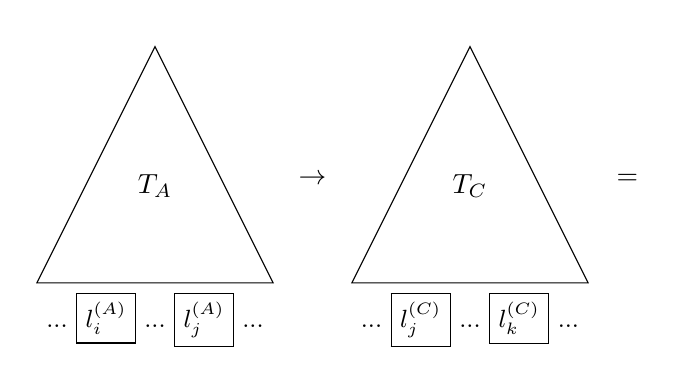
\begin{tikzpicture}
			\draw (1.5,1.5) node[anchor=north]{$T_A$};
			\draw (1.5,0) node[anchor=north]{\small$... \ \fbox{$l^{(A)}_i$} \ ... \ \fbox{$l^{(A)}_j$} \ ...$};
			\draw (0,0) node[anchor=north]{}
			-- (3,0) node[anchor=north]{}
			-- (1.5,3) node[anchor=south]{}
			-- cycle;
			\draw (3.5,1.5) node[anchor=north]{$\rightarrow$};
			\draw (5.5,1.5) node[anchor=north]{$T_C$};
			\draw (5.5,0) node[anchor=north]{\small$... \ \fbox{$l^{(C)}_j$} \ ... \ \fbox{$l^{(C)}_k$} \ ...$};
			\draw (4,0) node[anchor=north]{}
			-- (7,0) node[anchor=north]{}
			-- (5.5,3) node[anchor=south]{}
			-- cycle;
			\draw (7.5,1.5) node[anchor=north]{$=$};
	\end{tikzpicture}}
	\scalebox{.7}{
		\begin{tikzpicture}
			\draw (4,5.5) node[anchor=north]{$T_A$};
			\draw (4,4) node[anchor=north]{\small$... \ \dbox{$l^{(A)}_i$} \ ................................. \ \dbox{$l^{(A)}_j$} \ ...$};
			\draw (1,4) node[anchor=north]{}
			-- (7,4) node[anchor=north]{}
			-- (4,7) node[anchor=south]{}
			-- cycle;
			\draw (1.25,1.5) node[anchor=north]{$T_C \cap l^{(A)}_i$};
			\draw (1,0) node[anchor=north]{\footnotesize$l^{(C)}_i\cap l^{(A)}_i \ ... \ \fbox{$l^{(C)}_j \cap l^{(A)}_i$} \ ... \ \fbox{$l^{(C)}_k \cap l^{(A)}_i$}$};
			\draw (-1.5,0) node[anchor=north]{}
			-- (3.5,0) node[anchor=north]{}
			-- (1.75,3) node[anchor=south]{}
			-- cycle;
			\draw (6.75,1.5) node[anchor=north]{$T_C \cap l^{(A)}_j$};
			\draw (7,0) node[anchor=north]{\footnotesize$l^{(C)}_i \cap l^{(A)}_j \ ... \ \fbox{$l^{(C)}_j \cap l^{(A)}_j$} \ ... \ \fbox{$l^{(C)}_k \cap l^{(A)}_j$}$};
			\draw (4.5,0) node[anchor=north]{}
			-- (9.5,0) node[anchor=north]{}
			-- (6.25,3) node[anchor=south]{}
			-- cycle;
	\end{tikzpicture}}
	\caption[]{Schema of the derivation of a conditional Qtree. Nodes in \setlength{\fboxsep}{1pt}\dbox{dashed boxes} refer to the nodes that were verifying in the input antecedent Qtree, but are no longer verifying in the output conditional Qtree. Nodes in \setlength{\fboxsep}{1pt}\fbox{solid boxes} refer to the nodes that were verifying in the input consequent Qtree, and are thus still verifying in the output conditional Qtree.}\label{fig2:conditional-qtree-schema}
\end{figure} 


Second, the Node-Qtree intersection operation ($N\cap T$), which is part of the conditional Qtree formation process, is ``vacuous'' iff $N$ entails a specific leaf in $T$. We call the operation $N \cap T$ vacuous if it outputs $N$; the status of $N$ as verifying still depends on $T$'s verifying nodes. This is exemplified in Figure (\ref{fig2:vacuous-tree-node-inter}) assuming the node $N$ intersecting the Qtree entails (i.e. is a subset of) the leaf labeled $L$ in $T$. What happens is the following. The definition of a Qtree (see (\ref{ex2:qtree-def})) states that each intermediate node is partitioned by the set of its children. A corollary of this definition, is that, given a leaf $L$, all the nodes present on the path from $L$ to the root will be supersets of $L$, while all the other nodes will have no overlap with $L$. So, if $N \subseteq L$, $N$ will be a subset of all the nodes in $L$'s path to the root, and have no overlap with the other nodes, as well. Performing $N \cap T$ will thus initially yield a tree with same structure as the input Qtree $T$, but with nodes equal to $N$ along the path between the root and $L$'s original position, and empty nodes in all other positions. The Qtree reduction process devised in (\ref{ex2:qtree-reduction}) then removes all these empty nodes, and collapses the path made of $N$-nodes into one single node, namely, $N$. The whole operation therefore returns the input node $N$. Because the status of being a verifying node percolates when reduction takes place, as per (\ref{ex2:n-t-inter}), the output $N$ will be verifying iff $L$ was in $T$.



\begin{figure}[H]
	\centering
	\begin{minipage}[c]{.45\linewidth}
		\centering
		\begin{forest}
			[N$\cap$A[N$\cap$B[N$\cap$E][N$\cap$F]][N$\cap$C][N$\cap$D[N$\cap$G[N$\cap$J][N$\cap$K][N$\cap$L]][N$\cap$H][N$\cap$I]]]
		\end{forest}
	\end{minipage}
	\begin{minipage}[c]{.05\linewidth}
		\centering
		$\stackrel{N \subseteq K}{=}$
	\end{minipage}
	\begin{minipage}[c]{.25\linewidth}
		\centering
		\begin{forest}
			[N[$\emptyset$[$\emptyset$][$\emptyset$]][$\emptyset$][N[N[$\emptyset$][$\emptyset$][N]][$\emptyset$][$\emptyset$]]]
		\end{forest}
	\end{minipage}
	\begin{minipage}[c]{.1\linewidth}
		\centering
		$\stackrel{(\text{\ref{ex2:qtree-reduction}})}{=}$ N
	\end{minipage}
	\caption{Vacuous Node-Qtree intersection if $N$ entails a leaf of $T$, e.g. $K$.}\label{fig2:vacuous-tree-node-inter}
\end{figure}

The whole conditional Qtree formation process will then be vacuous if each verifying leaf in the antecedent Qtree entails a specific leaf of the consequent Qtree. Moreover, if each verifying leaf in the antecedent Qtree entails a specific \textit{non-verifying} leaf of the consequent Qtree, the output Qtree will be structurally identical to the antecedent Qtree but, will be left with \textit{no} verifying node. Such a tree will be deemed ill-formed as per principle (\ref{ex2:vacuous-flagging}). \\

We are now equipped to build conditional Qtrees from the sentences $S_{p}$=\textit{Ido is at SuB}, $\neg S_{p}$=\textit{Ido is not at SuB}, $S_{q}$=\textit{Ido is in Cambridge}, and $\neg S_{q}$=\textit{Ido is not in Cambridge}, whose Qtrees where computed in the previous Sections. This is done for $\neg S_p \rightarrow S_q$ in Figure \ref{fig2:qtrees-nptq}, using Qtrees for $\neg S_p$ from Figure \ref{fig2:qtrees-np} and Qtrees for $S_q$ from Figure \ref{fig2:qtrees-q}. Figure \ref{fig2:qtrees-nqtp}, does the same for $\neg S_q \rightarrow S_p$, just swapping the roles of $p$ and $q$. It is worth noting that the Qtrees in Figure (\ref{fig2:qtree-nptq-wh}) and (\ref{fig2:qtree-nqtp-wh}) are structurally identical to the antecedent Qtree used to build them. Such Qtrees are thus examples of a vacuous application of the Node-Qtree intersection operation. Their verifying nodes are however different from those of their antecedent Qtree, since, by definition, they are inherited from their consequent Qtree. 

\begin{figure}[H]
	\centering
	\begin{subfigure}[b]{.3\linewidth}
		\centering
		\scalebox{1}{
			\begin{forest}
				[CS [{$\p$}][\dbox{$\neg \p$} [\fbox{$\q$}][$\neg \q \cap \neg \p$]]]
			\end{forest}
		}
		\caption{Figure (\ref{fig2:qtree-np-polar}) $\rightarrow$ Figure (\ref{fig2:qtree-q-polar})}\label{fig2:qtree-nptq-polar-polar}
	\end{subfigure}\hfill
	\begin{subfigure}[b]{.3\linewidth}
		\centering
		\scalebox{1}{
			\begin{forest}
				[CS [{$\p$}][\dbox{$\neg \p$} [\fbox{$\q$}][$\r$][...]]]
			\end{forest}
		}
		\caption{Figure (\ref{fig2:qtree-np-polar}) $\rightarrow$ Figure (\ref{fig2:qtree-q-wh})}\label{fig2:qtree-nptq-polar-wh}
	\end{subfigure}\hfill
	\begin{subfigure}[b]{.3\linewidth}
		\centering
		\scalebox{1}{
			\begin{forest}
				[CS [{$\p$}][\fbox{$\q$}][\dbox{$\r$}][\dbox{...}]]
			\end{forest}
		}
		\caption{Figure (\ref{fig2:qtree-np-wh}) $\rightarrow$ Figure (\ref{fig2:qtree-q-polar})/(\ref{fig2:qtree-q-wh})\footnotemark}\label{fig2:qtree-nptq-wh}
	\end{subfigure}
	\caption[]{Qtrees for $\neg S\protect_{\p} \rightarrow S\protect_{\q} =$ \textit{If Ido is not at SuB then he is in Cambridge}. Nodes in \setlength{\fboxsep}{1pt}\dbox{dashed boxes} refer to the nodes that were verifying in the input antecedent Qtree, but are no longer verifying in the output conditional Qtree. Nodes in \setlength{\fboxsep}{1pt}\fbox{solid boxes} refer to the nodes that were verifying in the input consequent Qtree, and are thus still verifying in the output conditional Qtree.}
	\label{fig2:qtrees-nptq}
\end{figure}
\footnotetext{This Qtree is derived \textit{via} intersection and reduction as defined in (\ref{ex2:n-t-inter}). The Qtree derived \textit{before} reduction is given in (\ref{fig2:qtree-nptq-wh-before-reduc}). Reduction on this Qtree collapses the two $q$-nodes and makes the resulting node verifying; collapses the two $r$-nodes and makes the resulting node non-verifying; and so on for all other nodes different from the $p$-node.
	\begin{exe}
		\ex {\scalebox{.6}{
				\begin{forest}
					[CS [{$p$}][\dbox{$q$} [\fbox{q}]][\dbox{$r$} [r]][\dbox{...} [...]]]
		\end{forest}}}\label{fig2:qtree-nptq-wh-before-reduc}
	\end{exe}
}\label{fn:qtree-reduc}

\begin{figure}[H]
	\centering
	\begin{subfigure}[b]{.3\linewidth}
		\centering
		\scalebox{1}{
			\begin{forest}
				[CS [{$\q$}][\dbox{$\neg \q$} [\fbox{$\p$}][$\neg \p \cap \neg \q$]]]
			\end{forest}
		}
		\caption{Figure (\ref{fig2:qtree-nq-polar}) $\rightarrow$ Figure (\ref{fig2:qtree-p-polar})}\label{fig2:qtree-nqtp-polar-polar}
	\end{subfigure}\hfill
	\begin{subfigure}[b]{.3\linewidth}
		\centering
		\scalebox{1}{
			\begin{forest}
				[CS [{$\q$}][\dbox{$\neg \q$} [\fbox{$\p$}][$\r$][...]]]
			\end{forest}
		}
		\caption{Figure (\ref{fig2:qtree-nq-polar}) $\rightarrow$ Figure (\ref{fig2:qtree-p-wh})}\label{fig2:qtree-nqtp-polar-wh}
	\end{subfigure}\hfill
	\begin{subfigure}[b]{.3\linewidth}
		\centering
		\scalebox{1}{
			\begin{forest}
				[CS [{$\q$}][\fbox{$\p$}][\dbox{$\r$}][\dbox{...}]]
			\end{forest}
		}
		\caption{Figure (\ref{fig2:qtree-nq-wh}) $\rightarrow$ Figure (\ref{fig2:qtree-p-polar})/(\ref{fig2:qtree-p-wh})}\label{fig2:qtree-nqtp-wh}
	\end{subfigure}
	\caption[]{Qtrees for $\neg S\protect_{\q} \rightarrow S\protect_{\p} =$ \textit{If Ido is not in Cambridge then he is at SuB}; obtained \textit{mutatis mutandis} from Figure \ref{fig2:qtrees-nptq}}
	\label{fig2:qtrees-nqtp}
\end{figure}

At that point, we can already observe that Qtrees built from $\neg S_{p} \rightarrow S_q$, do not flag the $p$-node as verifying, since this corresponds to falsifying the antecedent of the conditional, a strategy that is typically overlooked. This feature of the model will be crucial in deriving the felicity of (\ref{ex2:pv(nptq)}): because $p$ is not treated as verifying in the Qtrees in Figure \ref{fig2:qtrees-nptq}, it will be possible to disjoin them with a Qtree for $S_p$, without producing redundant Qtrees as output. To clarify this intuition, we proceed to defining disjunction over Qtrees.






\section{Conclusion}


Unlike inquisitive semantics \citep{Mascarenhas2008,Ciardelli2009,Groenendijk2009,Ciardelli2018}, which proposes an \textit{unified} view of questions and assertions at the semantic level, what we propose here is a form of inquisitive \textit{pragmatics}: sentences are still assigned ``standard'' extensional/intensional meaning, but also have an inquisitive contribution at the pragmatic level. In fact, the current machinery may be closer in spirit to Dynamic Semantics \citep{Heim1983a,Heim1983b}, where different operators give rise to different incremental updates of the Context Set. Under our view, different operators will give rise to different \textit{parses} of the Context Set, at the inquisitive level. This will eventually allow to capture a contrast between (\ref{ex2:red-followup}) and (\ref{ex2:non-red-followup}).





